% ----------------------------------------------------------------------
%                   LATEX TEMPLATE FOR PhD THESIS
% ----------------------------------------------------------------------

% based on Harish Bhanderi's PhD/MPhil template, then Uni Cambridge
% http://www-h.eng.cam.ac.uk/help/tpl/textprocessing/ThesisStyle/
% corrected and extended in 2007 by Jakob Suckale, then MPI-CBG PhD programme
% and made available through OpenWetWare.org - the free biology wiki


%: Style file for Latex
% Most style definitions are in the external file PhDthesisPSnPDF.
% In this template package, it can be found in ./Latex/Classes/
\documentclass[oneside,11pt]{Latex/Classes/PhDthesisPSnPDF}

% Macro file for Latex
% Macros help you summarise frequently repeated Latex commands.
% Here, they are placed in an external file /Latex/Macros/MacroFile1.tex
% An macro that you may use frequently is the figuremacro (see introduction.tex)
% This file contains macros that can be called up from connected TeX files
% It helps to summarise repeated code, e.g. figure insertion (see below).

% produce an unit vector
\newcommand{\unitvector}[1]{\ensuremath{\hat{\mathbf{#1}}}}
% produce the normal vector
\newcommand{\normal}{\ensuremath{\hat{\mathbf{n}}}}
%\newcommand{\unitvector}[2]{\ensuremath{\hat{\mathbf{#1}}_{#2}}}
\newcommand{\point}[1]{\ensuremath{\mathbf{#1}}}
\newcommand{\pointi}[2]{\ensuremath{\mathbf{#1}_{#2}}}
%put figure and table in multicols environment.
\makeatletter
\newenvironment{tableInMulticols}
  {\def\@captype{table}}
  {}

\newenvironment{figureInMulticols}
  {\def\@captype{figure}}
  {}
\makeatother

% insert a centered figure with caption and description
% parameters 1:filename, 2:title, 3:description and label
\newcommand{\figuremacro}[3]{
	\begin{figure}[htbp]
		\centering
		\includegraphics[width=1\textwidth]{#1}
		\caption[#2]{\textbf{#2} - #3}
		\label{#1}
	\end{figure}
}

% insert a centered figure with caption and description AND WIDTH
% parameters 1:filename, 2:label, 3:caption, 4: textwidth
% textwidth 1 means as text, 0.5 means half the width of the text
\newcommand{\figuremacroW}[4]{
	\begin{figure}[htbp]
		\centering
		\includegraphics[width=#4\textwidth]{#1}
		\caption{#3}
		\label{#2}
	\end{figure}
}

% inserts a figure with wrapped around text; only suitable for NARROW figs
% o is for outside on a double paged document; others: l, r, i(inside)
% text and figure will each be half of the document width
% note: long captions often crash with adjacent content; take care
% in general: above 2 macro produce more reliable layout
\newcommand{\figuremacroN}[3]{
	\begin{wrapfigure}{o}{0.5\textwidth}
		\centering
		\includegraphics[width=0.48\textwidth]{#1}
		\caption[#2]{{\small\textbf{#2} - #3}}
		\label{#1}
	\end{wrapfigure}
}

% predefined commands by Harish
\newcommand{\PdfPsText}[2]{
  \ifpdf
     #1
  \else
     #2
  \fi
}

\newcommand{\IncludeGraphicsH}[3]{
  \PdfPsText{\includegraphics[height=#2]{#1}}{\includegraphics[bb = #3, height=#2]{#1}}
}

\newcommand{\IncludeGraphicsW}[3]{
  \PdfPsText{\includegraphics[width=#2]{#1}}{\includegraphics[bb = #3, width=#2]{#1}}
}

\newcommand{\InsertFig}[3]{
  \begin{figure}[!htbp]
    \begin{center}
      \leavevmode
      #1
      \caption{#2}
      \label{#3}
    \end{center}
  \end{figure}
}


%%% Local Variables:
%%% mode: latex
%%% TeX-master: "~/Documents/LaTeX/CUEDThesisPSnPDF/thesis"
%%% End:


\DeclareMathAlphabet{\mathcal}{OMS}{cmsy}{m}{n}

%glossary ralated code
\usepackage[toc]{glossaries}
\renewcommand*{\glossaryentrynumbers}[1]{}
%\setlength{\glsdescwidth}{0.8\linewidth}
\makeglossaries

\glossarystyle{list}
\renewcommand*{\glsgroupskip}{}

\addbibresource[]{bibliography.bib}


% this file is called up by thesis.tex
% content in this file will be fed into the main document

% 1 = Entry name, e.g. abbreviation; 2 = Explanation
% You can place all explanations in this separate file or declare them in the middle of the text. Either way they will be collected in the glossary.

% required to print nomenclature name to page header
\newacronym{SLAM}{SLAM}{Simultaneous Localization And Mapping}
\newacronym{LRF}{LRF}{Laser Range Finder}
\newacronym{aLRF}{aLRF}{actuated Laser Range Finder}
\newacronym{NBV}{NBV}{Next Best Viewpoint}
\newacronym{FoV}{FoV}{Field of View}
\newacronym{ToF}{ToF}{Time of Flight}
%\newacronym{NNS}{NNS}{Nearest Neighbor Search}
\newacronym{EGI}{EGI}{Extended Gaussian Image}
%\newacronym{PCA}{PCA}{Principal Component Analysis}
\newacronym{MSE}{MSE}{Mean Square Error}
\newacronym{ICP}{ICP}{Iterative Closest Point}
\newacronym{NDT}{NDT}{Normal Distributions Transform}
\newacronym{3D-NDT}{3D-NDT}{Three-Dimensional Normal Distributions Transform}
\newacronym{MUMC}{MUMC}{Minimum Uncertainty Maximum Consensus}
\newacronym{IMU}{IMU}{Inertial Measurement Units}
\newacronym{GNSS}{GNSS}{Global Navigation Satellite Systems}
%\newacronym{EKF}{EKF}{Extended Kalman Filter}
%\newacronym{MLS}{MLS}{Multi-Level Surface}
\newacronym{PDF}{PDF}{Probability Density Functions}
%\newacronym{MLE}{MLE}{Maximum-Likelihood Estimation}
%\newacronym{P2D}{P2D}{Point-to-Distribution}
%\newacronym{FPFH}{FPFH}{Fast Point Feature Histograms}
%\newacronym{DIFT}{DIFT}{Depth-interpolated Image FeaTures}
\newacronym{RANSAC}{RANSAC}{RANdom SAmple Consensus}
\newacronym{SVM}{SVM}{Support Vector Machine}
\newacronym{PTU}{PTU}{Pan-Tilt Unit}
\newacronym{FILO}{FILO}{First-In-Last-Out}


%: ----------------------------------------------------------------------
%:                  TITLE PAGE: name, degree,..
% ----------------------------------------------------------------------
\ifpdf
    \pdfinfo { /Title  (PhD Thesis)
               /Creator (TeX)
               /Producer (pdfTeX)
               /Author (Sarah Fritzsche)
               /CreationDate (D:20140120)  %format D:YYYYMMDDhhmmss
               /ModDate (D:20140502)
               /Subject (SubectText)
               /Keywords (Musiktherapie, COPD) }
    \pdfcatalog { /PageMode (/UseOutlines)
                  /OpenAction (fitbh)  }
\fi

% ----------------------------------------------------------------------


\hyphenation{Sym-pa-tho-mi-me-ti-ka}
%\hyphenation{ent-"undungs-hemmende}
%\hyphenation{Ganz-k"or-per-ple-thys-mo-gra-phie}

\setlength{\skip\footins}{0.5cm} % space between text body and footnote line

% turn of those nasty overfull and underfull hboxes
\hbadness=10000
\hfuzz=50pt
%: --------------------------------------------------------------
%:                  FRONT MATTER: dedications, abstract,..
% --------------------------------------------------------------
%\makeglossaries
\begin{document}
% sets line spacing
\renewcommand\baselinestretch{1.0}
\baselineskip=14pt plus1pt

%: ----------------------- generate cover page ------------------------

\maketitle  % command to print the title page with above variables

%: ----------------------- tie in front matter ------------------------
%\frontmatter
%\reviewers
%% Thesis Dedictation ---------------------------------------------------

\begin{dedication} %this creates the heading for the dedication page

To my family...

\end{dedication}

% ----------------------------------------------------------------------
%\phantomsection
\chapter*{Change list}
\markboth{\MakeUppercase{Change list}}{}
\addcontentsline{toc}{chapter}{Change list}

\begin{itemize}
 \item Figure 3.2(b), the horizontal field of view has been corrected to 360 degrees.
 \item Algorithm 4.4, line 1, duplicate of Q <-- emptyset.
\end{itemize}
%% Thesis Acknowledgements ------------------------------------------------
\phantomsection
\chapter*{Acknowledgements}
\markboth{\MakeUppercase{Acknowledgements}}{}
\addcontentsline{toc}{chapter}{Acknowledgements}

\if0
Doing a PhD was a long and exciting journey, which would not be possible without the help and support of many people. First of all I am most grateful to my supervisor Prof. Dr. Jianwei Zhang for giving me the opportunity to pursue a PhD at the University of Hamburg and providing me such a good and liberal academic environment. 

Next, I would like to extend my thanks to my daily supervisor and good friend Prof. Dr. Houxiang Zhang, whose support was always there for both technical and personal problems, not only in the first two years of my study when he was in Hamburg, but also for the second two years after he moved to {\AA}lesund. His constructive criticism helped focus my ideas and his constant encouragement kept me going in spite of many stumbling blocks on the road.    

Writing a dissertation is no easy task, but the same can be said of reviewing it. I would like to thank all the people who helped by reviewing parts of this work, especially my external reviewers --- Prof. Dr. Reinhard Koch and Dr. Peer Stelldinger. 

%I have to say, without your encouragement, I was almost going to drop when the traffic accident came to me while I had been ill for a long time. 

All the members of our TAMS group are greatly acknowledged, the time spent with you was wonderful. I own a great deal to Tatjana (Lu) Tetsis, thank you for helping me so much during the past time. My sincere thanks also go to Benjamin Adler for always being excited about my problems and ideas, always sharing his ideas with me, and the engaging discussions we had during and after work. 

I am grateful to my former colleagues from NuBot, Huimin Lu, Xiangke Wang, and Shaowu Yang are especially acknowledged, thanks a lot for valuable comments and suggestions on my conference and journal papers, as well as this dissertation. 

%I am thankful to all the people who helped by reviewing this work, they are Dr. Norman Hendrich, Shaowu Yang, Benjamin Adler, Weiwei Kong, and Jie Liang; especially my external reviewers --- Prof. Dr. Reinhard Koch and Dr. Peer Stelldinger.   

Being away from my family was not easy, however, many friends from Hamburg and other places provided another family away from home. I own special thanks to all of my friends. In this regard, Jianhua Zhang, Guoyuan Li, Gang Cheng, Bo Sun, and Weiwei Kong deserve special mention.

Finally, I would like to thank the people closest to me for their love and support --- my parents and brother, my girl friend Fang, especially to my little nephew who brings a lot of happy moments.  
\fi
% ------------------------------------------------------------------------

\vspace*{5mm}

\hfill Benjamin Adler

\hfill Hamburg, May 2014

%\phantomsection
\chapter*{Abstract}
\markboth{\MakeUppercase{Abstract}}{}
\addcontentsline{toc}{chapter}{Abstract}

This paper introduces a custom-built unmanned aerial vehicle, capable of autonomous exploration in urban environments. It consists of a multicopter, an inertial navigation system and two 2D laser range finders. In addition to a description of the hardware architecture and individual components being used, the authors also discuss challenges and problems that arose during its construction as well as optimizations and workarounds applied in the course of its development.

Also presented is the software architecture, with a focus on a novel algorithm capable of generating multiple next best views (NBVs), sorted by achievable information gain. Although being designed for application on airborne platforms in urban environments, it works directly on raw point clouds and thus can be used with any sensor generating spatial occupancy information (e.g. LIDAR, RGBD- or time-of-flight-cameras). To satisfy constraints introduced by real-time operation on UAVs, the algorithm is implemented on a highly parallel SIMD architecture and benchmarked using GPUs from multiple hardware generations, using data from real flights. It is also compared against the previous, CPU-based proof of concept.

As the underlying hardware imposes limitations with regards to memory access and concurrency, necessary data structures and further performance considerations are explained in detail.

Open-source code for this paper is available at http://www.github.com/benadler/octocopter/.
%\phantomsection
\chapter*{Kurzfassung}
\markboth{\MakeUppercase{Kurzfassung}}{}
\addcontentsline{toc}{chapter}{Kurzfassung}

Die vorliegende Dissertation behandelt ...
%: ----------------------- contents ------------------------
\setcounter{secnumdepth}{3} % organisational level that receives a numbers
\setcounter{tocdepth}{3}    % print table of contents for level 3
\tableofcontents            % print the table of contents
\addtocontents{toc}{\protect{\pdfbookmark[0]{\contentsname}{toc}}}
% levels are: 0 - chapter, 1 - section, 2 - subsection, 3 - subsection
%: ----------------------- list of figures/tables ------------------------
%\listoffigures	% print list of figures
%\newpage\thispagestyle{empty}
%\listoftables  % print list of tables
%\newpage\thispagestyle{empty}

%\glsaddall
%\printglossaries
%\newpage\thispagestyle{empty}


\begin{multicols}{2} % \begin{multicols}{#columns}[header text][space]
\begin{footnotesize} % scriptsize(7) < footnotesize(8) < small (9) < normal (10)
\printnomenclature[1.5cm] % [] = distance between entry and description
\label{nom} % target name for links to glossary

\end{footnotesize}
\end{multicols}

%: --------------------------------------------------------------
%:                  MAIN DOCUMENT SECTION
% --------------------------------------------------------------

% the main text starts here with the introduction, 1st chapter,...
\mainmatter
%: ----------------------- subdocuments ------------------------
% Parts of the thesis are included below. Rename the files as required.
% But take care that the paths match. You can also change the order of appearance by moving the include commands.

\begin{spacing}{1.5}

%: ----------------------- introduction file header -----------------------
\chapter{Einleitung}
%\epigraph{Pommes sind lecker.}{Ben}
% the code below specifies where the figures are stored
\ifpdf
    \graphicspath{{1_introduction/figures/PNG/}{1_einleitung/figures/PDF/}{1_einleitung/figures/}}
\else
    \graphicspath{{1_einleitung/figures/EPS/}{1_einleitung/figures/}}
\fi

% ----------------------------------------------------------------------
%: ----------------------- introduction content -----------------------
% ----------------------------------------------------------------------


While robots ...

\begin{quote}
``It is not that difficult to build computers capable of playing chess or doing sums. Computers find it easy to do what we learned at school. But computers have a very hard time learning what children learn \textit{before} they start school: [...] navigating a backyard, recognizing a face; seeing.'' 
\end{quote}

\begin{itemize}
\item der erste Punkt
\item der zweite Punkt
\end{itemize}

\begin{enumerate}
\item der erste Punkt
\item der zweite Punkt
\end{enumerate}

\section{Motivation} % section headings are printed smaller than chapter names
\lettrine{H}{uman} beings have been dreaming to create intelligent \emph{robots} 

\subsection{Untergedängs}
tüdlötß
\subsubsection{unteruntergedaengs}
hehe

\paragraph{hahaha parapgrah}

\section{Outline}
\indent{The rest of this thesis is organized as follows: }

Chapter \ref{chapter:soa} 

\section{Research questions and contributions}
\label{sec:introduction:contributions}

\newpage\thispagestyle{empty}
\ifpdf
\graphicspath{{2_chronisch_obstruktive_lungenerkrankung/figures/PNG/}{2_chronisch_obstruktive_lungenerkrankung/figures/PDF/}{2_chronisch_obstruktive_lungenerkrankung/figures/}}
\else
    \graphicspath{{2_chronisch_obstruktive_lungenerkrankung/figures/EPS/}{2_chronisch_obstruktive_lungenerkrankung/figures/}}
\fi

\chapter{Chronisch obstruktive Lungenerkrankung (COPD)}
\label{chapter:copd}

Die Chronisch obstruktive Lungenerkrankung, auf englisch Chronic Obstructive Pulmonary Disease (COPD) genannt, ist trotz ihrer starken Verbreitung noch vielen Menschen nicht bekannt.
Bei der COPD handelt es sich um eine chronische Lungenkrankheit mit progredienter Atemwegsverengung; sie gilt als die häufigste Erkrankung der Atmungsorgane. COPD ist ein Sammelbegriff für die chronisch obstruktive Bronchitis und das Lungenemphysem, welche entweder einzeln oder gemeinsam auftreten \autocite[vgl.][153]{lorenz2009}.  Die COPD resultiert aus einer langfristigen Entzündung der Atemwege, welche durch ständige Belastung mit in erster Linie Zigarettenrauch, aber auch Umweltfaktoren, Staubpartikeln und giftigen Dämpfen entsteht. Ätiologisch wird davon ausgegangen, dass 80-90\% der COPD-Patienten die Erkrankung aufgrund von Nikotinabusus entwickelt haben; das sind in etwa 15\% der Zigarettenraucher\autocite[vgl.][154]{lorenz2009}. 

Als ein wichtiges Diagnosemerkmal gilt die Atemnot (Dispnoe), welche aus der Obstruktion der Bronchien resultiert. Diese wird durch drei Faktoren ausgelöst: 

\begin{enumerate}
\item Verkrampfung der Bronchialmuskulatur (Bronchospasmus)
\item Anschwellen der Schleimhaut in den Bronchien (Ödem)
\item Krankhaft erhöhte Schleimproduktion (Hyperkrinie) aufgrund einer dauerhaften Entzündung der Atemwege (chronische Bronchitis)
\end{enumerate}

Durch die Hyperkrenie werden die Zilien - kleine Flimmerhärchen in den Bronchien - immer mehr daran gehindert, Schadstoffe aus der Lunge hinaus zu befördern, da ihre Bewegungsfähigkeit eingeschränkt wird. Dieser Prozess führt über einen längeren Zeitraum zur Zerstörung der Flimmerhärchen und somit zu einem größeren Exazerbationsrisiko (siehe unten).
Die Luftnot tritt im Anfangsstadium nur unter Belastung auf, später auch im Ruhezustand \autocite[vgl.][6f.]{lorenz2009}. Die allgemeine Symptomatik umfasst morgendlichen Kopfschmerz, Gewichtsverlust, welcher auf verstärkte Atemarbeit und systemische Entzündungsreaktionen zurückzuführen ist, zunehmenden Leistungsabfall, Einflussstauung, Ödeme der unteren Extremitäten und weiter abnehmende Belastbarkeit aufgrund des s.g. Cor pulmonale (Lungenherz, s. weiter unten).
Eine chronisch obstruktive Lungenerkrankung liegt laut WHO-Definition dann vor, wenn sowohl Husten und Auswurf über wenigstens als 3 Monate in mindestens 2 aufeinander folgenden Jahren bestehen und somit als chronisch anzusehen sind, als auch andere Krankheiten wie z.B. Bronchiektasen, Staubbelastung, cystische Fibrose, Asthma, Fremdkörper u.a. im Vorfeld ausgeschlossen werden konnten \autocite[vgl.][71]{koehler2010}. 

%todo Grafik der Lunge als auch der Lungenbläschen

Das Lungenemphysem ist das Resultat länger andauernder Entzündungsreaktionen auf o.g. mögliche externe Partikel. Durch entzündliche Prozesse  werden die Zellwände in den Alveolen  (Lüngenbläschen, siehe Abbildung todo) zerstört. Hierfür sind Proteasen zuständig, die bei Eindringen von schädlichen Stoffen in die Lunge durch das Immunsystem freigesetzt werden. So genannte Antiproteasen können jedoch vor der Zerstörung der Alveolarwände schützen. Diese werden für normal körpereigen produziert; hierzu gehört u.a. das Alpha-1-Antitripsin. Einige Patienten leiden jedoch unter einem genetische bedingen Alpha-1-Antripsinmangel, wodurch ein erhöhtes Risiko für die Ausbildung eines Lungenemphysems besteht.
Das bedeutet, dass sich mit weiterbestehender Entzündung die Anzahl der für den Sauerstoff-Kohlendioxid-Austausch notwendigen Alveolen verringert und sich die Lufträume in der Lunge vergrößern. Dadurch wird nach und nach die Lungenelastizität eingeschränkt, was eine Überdehnung der Lunge (Hyperinlation) mit Minderdurchblutung und einem irreversiblen Schwund an Lungengewebe als auch eine Einschränkung der Atemfunktion nach sich zieht. Dies geschieht jedoch nicht nur durch die degenerativen Prozesse in einem Lungenlappen, sondern auch durch funktionelle Beeinträchtigung anderer umliegender, gesunder Lungenlappen aufgrund der partiellen Überblähung. Auch andere Organe können möglicherweise beschädigt werden. Denn bei Nichtbehandlung des Emphysems kommt es zu einer erhöhten Pumpleistung des Herzmuskels und so über längere Zeit zu einer Schädigung desselben, da dieser nun mehr Blut transportieren muss, um die Organe ausreichend mit Sauerstoff zu versorgen. Daher ist die Todesursache bei einem Lungenemphysem in den meisten Fällen ein Herzversagen und nicht, wie evtl. zuvor vermutet, Erstickung.

Bei Fortschreiten der COPD kommt es immer wieder zu Exazerbationen, das heißt zu akuten Verschlechterungen der alltäglichen Krankheitssymptome, was zu Symptomen wie Atemnot, Husten, vermehrter Sputummenge oder Fieber führen kann. Sie resultieren zu 60-70\% aus einer Infektion der Lunge oder nichtinfektiösen Ursachen wie akuter Luftverschmutzung oder Verschlechterung von Begleiterkrankungen und sollten daher zeitnah behandelt werden.

Das Auftreten der COPD nimmt mit dem Alter zu, dabei kommt es ab dem 50. Lebensjahr zu einem rapiden Anstieg der Prävalenz. Im siebten Dezennium ist die Spitze des Auftretens mit etwa 10\% bei Männern und ca. 5\% bei Frauen erreicht\autocite[vgl.][153]{lorenz2009}. Nach Köhler/Schönhofer/Voshaar sei Vorsicht geboten bei dem Einbezug von Statistiken in diesem Bereich, da die verfügbaren Daten zur Prävalenz der COPD sehr von dem untersuchten Kollektiv bzw. den Altersgruppen abhängen (2010: 72). Insgesamt gehen sie jedoch von folgenden Zahlen aus: Etwa 10\% der deutschen Bürger ab dem 40. Lebensjahr seien davon betroffen, wobei ca. 10\% dieser Patientenkohorte einen höheren Schweregrad aufweisen. Es wird davon ausgegangen, dass den Hausärzten nur etwa bei der Hälfte der Patienten die Erkrankung bekannt ist.
In Bezug auf die Mortalität gilt bei ca. 3,5\% aller Todesfälle COPD als die Haupttodesursache. Allerdings ist sie bei ca. 4,5\% der Todesfälle mitverursachend. Es wird davon ausgegangen, dass COPD auf der Liste der häufigsten Todesursachen in den nächsten 6 Jahren weltweit von dem 4. auf den 3. Platz aufsteigen wird.
Laut der COPD-Leitlinie besteht eine hohe sozioökonomische Belastung durch die steigende Zahl an COPD-Fällen. In der Hochrechnung von Krankenhausstatistiken seit 1996 wurden für obstruktive Atemwegserkrankungen 2,7 Mio. Krankenhaustage erfasst. Einen Großteil macht hierbei die Behandlung chronischer Bronchitis und ihrer Folgen aus. Auch die von der AOK hochgerechneten jährlichen Krankheitstage in Höhe von 25 Mio. aufgrund der chronischen Bronchitis sind immens. Sie entsprechen volkswirtschaftlichen Gesamtkosten von etwa 5,93 Mrd. € jährlich \autocite[vgl.][e4]{vogelmeier2007}.

Um das Krankheitsbild, Diagnostik und Therapie weltweit zu vereinheitlichen, wurde der o.g. englische Begriff eingeführt. Eine globale Initiatve, welche 2001 von der Weltgesundheitsorganisation (WHO) und den National Institutes of Health (NIH) gegründet wurde, hat zusätzlich dazu beigetragen, dass weltweit eine einheitliche Leitlinie, die s.g. GOLD-Leitlinie, zum Tragen kommt. Die Erkrankung wird hiernach in vier Schweregrade eingeteilt, die sich an dem gemessenen Ausatemvolumen orientieren. Einige Autoren, darunter Köhler/Schönhofer/Voshaar \autocite[vgl.][75]{koehler2010}, bewerten diese Leitlinie jedoch als einen Rückschritt, da diese das Krankheitsbild in Bezug auf seine Pathophysiologie zu sehr vereinfache.

Diese Einteilung wird jedoch in der Praxis nach wie vor vorgenommen, weshalb sie an dieser Stelle dargestellt werden soll.

In den GOLD-Leitlinien wird zwischen 4 Stadien unterschieden. Für die Einteilung kommen 2 Werte der Lungenfunktionsprüfung (siehe \ref{diagnostik}) zum Tragen. Der erste Wert, das forcierte exspiratorische Volumen (FEV1) gibt Auskunft darüber, wieviel Luft eine Person innerhalb einer Minute forciert ausatmen kann. Für eine Einstufung wird der FEV1-Wert eines Patienten mit Soll- bzw. Normalwerten verglichen, welche wiederum abhängig von Geschlecht, Alter und Körpergröße des Patienten sind. Dieser Wert gilt in der Regel als Indikator für die Schwere der Erkrankung. In diesem Zusammenhang ist auch das Verhältnis zwischen der inspiratorischen Vitalkapazität (Einatemvolumen) und dem FEV1 für die Diagnosestellung wichtig (siehe Tabelle todo). Bei der leichtgradigen COPD (Schweregrad I) besteht die Atemwegsobstruktion ohne eine signifikante FEV1-Verminderung. Patienten in diesem Stadium berichten über chronischen Husten und Auswurf, bemerken jedoch meist noch keine Einschränkung ihrer Lungenfunktion. Beim Schweregrad II besteht neben der Atemwegsobstruktion bereits eine geringe FEV1- Verminderung und die kranksheitsspezifischen Symptome, insbesondere Dyspnoe unter Belastung, nehmen zu. Die schwere COPD (Schweregrad III) ist charakterisiert durch eine höhergradige FEV1-Verminderung, das heißt FEV1-Werten zwischen 30\% und 50\% des Soll. Es besteht jedoch nur eine geringe oder keine Korrelation zwischen dem Ausmaß der Dyspnoe und dem Schweregrad der Lungenfunktionseinschränkung. Für den Schweregrad IV gilt ein FEV1-Wert von todo kleiner=30\% Soll als ausschlaggebend. Bei einer gleichzeitigen respiratorischen Insuffizienz darf für die Einteilung in den Schweregrad IV der FEV1-Wert <50\% soll betragen \autocite[vgl.][e8]{vogelmeier2007}.

\begin{table}
\centering
\begin{tabular}{lp{10cm}}
	\textbf{Schweregrad} & \textbf{Kriterien} \\
	\hline \hline
	I (leicht) & $FEV_{1} \ge 80\% Soll, FEV_{1}/VC < 70\%$ \newline mit/ohne Symptomatik (Husten, Auswurf) \\
	\hline
	II (mittel) & $50\% Soll \le FEV_{1} < 80\% Soll, FEV_{1}/VC < 70\%$ \newline mit chronischen Symptomen/ohne chronische Symptome (Husten, Auswurf, Dyspnoe) \\
	\hline
	III (schwer) & $30\% Soll < FEV_{1} < 50\% Soll, FEV_{1}/VC < 70\%$ \newline mit chronischen Symptomen/ohne chronische Symptome (Husten, Auswurf, Dyspnoe) \\
	\hline
	IV (sehr schwer) & $FEV_{1} \le 30\% Soll, FEV_{1}/VC < 70\%$ oder \newline $FEV_{1} < 50\% Soll$ plus chronische respiratorische Insuffizienz \\
	\hline
\end{tabular}
\caption{Schweregradeinteilung der COPD, aus \autocite[e9]{vogelmeier2007}}
\label{tab:copd_schweregrade}
\end{table}

Eine neuere, multidimensionale Schweregradbeurteilung stellt der s.g. BODE-Index dar (siehe Anhang). Dieser bezieht in seine Bewertung den Body-mass-index (B), die FEV1-Einschränkung (O, Obstruction), das Dyspnoeempfinden (D) und die Belastbarkeit (E, exercise capacity) mit ein. Dabei wird eine Aussage über das Dyspnoeempfinden mittels des leicht abgeänderten Medical Research Council (MRC)-Scores vorgenommen, der folgendermaßen eingeteilt ist: "0 = keine Atemnot, 1 = Atemnot bei schwerer Belastung, 2 = Atemnot bei leichter Belastung, 3 = zu atemlos, das Haus zu verlassen und atemlos beim An- und Ausziehen" \autocite[186f.]{welte2007}. Die Belastbarkeit wird durch den 6-Minuten-Gehtest gemessen, welcher sich nach der zurückgelegten Strecke in m orientiert.


\section{Diagnostik} % section headings are printed smaller than chapter names
\label{diagnostik}
Um eine Verdachtsdiagnose stellen zu können, wird zu Beginn eine umfangreiche \emph{Anamnese} durchgeführt. Diese umfasst folgende, auf COPD verweisende Kriterien: Alter, Familienanamnese, Husten, Auswurf, Atemnot unter Belastung, Rauchgewohnheit und/oder inhalative Belastung am Arbeitsplatz, Anzahl der Exazerbationen pro Jahr, gegenwärtige Medikation, Beeinträchtigung im Alltag, Sozialanamnese, Störungen der Atmung im Schlaf, mögliche Komorbiditäten (s. weiter unten) und Gewichtsverlust. 

Folgende \emph{körperliche Untersuchungsbefunde} geben ebenfalls Hinweis auf eine mögliche COPD, wobei bei einer leichtgradigen Ausprägung der Erkrankung diese Befunde unauffällig sein können: bei einer mittelgradigen COPD deuten verlängertes Exspirium, Giemen, Pfeifen und Brummen auf eine Obstruktion der Atemwege, ein tief stehendes, wenig verschiebbares Zwerchfell und hypersonorer Klopfschall auf eine Lungenüberblähung hin. Für eine schwere Form der Erkrankung sind in der COPD-Leitlinie folgende Untersuchungsbefunde kennzeichnend:
\begin{itemize}
\item "Zeichen der chronischen Lungenüberblähung mit abgeschwächtem Atemgeräusch, leisen Herztönen, Fassthorax und inspiratorischen Einziehungen im Bereich der Flanken
\item pfeifende Atemgeräusche, insbesondere bei forcierter Exspiration
\item Zeichen der Sekretansammlung im Anhusteversuch
\item zentrale Zyanose
\item Konzentrationsschwäche und verminderte Vigilanz
\item Gewichtsverlust
\item periphere Ödeme
\item indirekte Zeichen der pulmonalen Hypertonie mit präkordialen Pulsationen, betontem Pulmonalklappenschlusston, einer Tricuspidalklappeninsuffizienz mit einem Systolikum über
dem 3. bzw. 4. ICR rechts parasternal." \autocite[e6]{vogelmeier2007}
\end{itemize}
Es müssen für eine COPD-Diagnosestellung jedoch nicht alle genannten Symptome vorliegen.

Einen sehr wichtigen Teil der Diagnostik stellen \emph{Lungenfunktionstestungen} dar, weil sie zum Einen für die Einteilung der Schweregrade gebraucht werden und andererseits Aussagen über eine nicht vollständig reversible Atemwegsobstruktion durch Nicht-Ansprechen auf die Gabe von Bronchodilatatoren und/oder Glukokortikoiden (siehe auch \ref{medikamentoese_therapien}) treffen können, was ein klares Indiz für eine ausgebildete COPD darstellt. Dieser Reversibilitätstest ist insbesondere für die Differenzialdiagnose zwischen Asthma und COPD entscheidend, welche für das Management der COPD sehr wichtig ist. Die charakteristischen Merkmale beider Erkrankungen sind in Tabelle todo gegenübergestellt.

Die gängigsten Lungenfunktionstests sind die Spirometrie und die Ganzkörperplethysmographie. Bei der Spirometrie wird durch Ein- und Ausatmen in ein hierfür spezialisiertes Gerät gemessen, wie viel Luft durch die Lunge aufgenommen und wie schnell diese gefüllt und wieder geleert werden kann. Hier wird sowohl der oben mehrmals erwähnte FEV1-Wert als auch die forcierte Vitalkapazität (FVC) ermittelt. Je niedriger der FEV1-Wert ausfällt, desto schlechter ist die Lungenkapazität. Bei der Ganzkörper-, auch Bodyplethysmographie genannt, wird hingegen gemessen, wieviel Luft in der Lunge nach der maximalen Ausatmung in der Lunge verbleibt. Das Ergebnis bildet sich in der s.g. funktionellen Residualkapazität (FRC) ab \autocite[vgl.][e6f.]{vogelmeier2007}. Bei einem Lungenemphysem wird das Residualvolumen größer sein als bei vergleichbaren gesunden Menschen. In bestimmten Fällen, wie bei Patienten mit einer Diskrepanz zwischen Dyspnoe und Einschränkung der FEV1 oder bei Patienten der Schweregrade III und IV, können zur weiteren Abklärung noch andere Messverfahren eingesetzt werden.

Ein weiteres Verfahren ist die \emph{arterielle Blutgasanalyse}, welche zur Abklärung einer Gasaustauschstörung, auch respiratorische (Partial-)Insuffizienz genannt, sowie zur therapeutischen Abschätzung der Indikation für eine Sauerstofftherapie dient. Die Bestimmung der Blutgase geschieht über Analyse von hyperämisiertem Kapillarblut, welches i.d.R. dem Ohrläppchen entnommen wird. "Eine respiratorische Partialinsuffizienz wird bei Sauerstoff-Partialdruck (PaO2)-Werten < 8,0 kPa (60 mmHg) diagnostiziert, eine Hyperkapnie bei einem CO2-Partialdruck (PaCO2) > 6,0 kPa [45 mm Hg]. Bei Patienten mit schwerer COPD kann eine respiratorische Globalinsuffizienz mit arterieller Hypoxämie und Hyperkapnie angetroffen werden" \autocite[190]{welte2007}.

Wie bereits oben erwähnt, gehören auch \emph{Belastungstests} zur COPD-Diagnostik. Diese sollen Aufschluss über die verschiedenen Ursachen der Belastungsdyspnoe und die Therapieeffekte von Medikamenten und Orientierung zur Erstellung eines individuell angepassten Trainingsprogramms im ambulanten als auch rehabilitativen Bereich geben \autocite[vgl.][e7]{vogelmeier2007}. 

\emph{Bildgebende Verfahren} sind für die Diagnostizierung eines Lungenemphysems sowie für die Differenzialdiagnostik (insbesondere zum Ausschluss eines Bronchialkarzinoms oder kardialer Erkrankungen) von großer Bedeutung. Hierfür werden i.d.R. Röntgenaufnahmen und Computertomografie (High Resolution, HR-CT) der Thoraxorgane eingesetzt. Die HR-CT wird insbesondere vor einer Resektion von Emphysem-Bullae (Emphysemblasen) oder einer Lungenvolumenreduktion (siehe \ref{nicht-medikamentoese_therapien}) durchgeführt \autocite[191]{welte2007}.

Bei Patienten mit häufigen Exazerbationen (>3 pro Jahr), Therapieversagern und/oder bei besonders schweren Erkrankungen, die auf eine multiresistente bakterielle Besiedelung der Lunge hindeuten, wird die \emph{Sputumdiagnostik} empfohlen. Patienten sind in der Regel in der Bewertung ihres eigenen Sputums, auch bekannt als Auswurf oder Sekret, geschult, um Veränderungen ihres Krankheitszustandes frühzeitig erkennen zu können. 

Zudem werden aufgrund des Zusammenhangs der COPD mit kardialer Belastung auch Echokardiographie und Elektrokardiogramm eingesetzt.

Da es sich bei der COPD um eine progrediente Erkrankung mit fließenden Übergängen handelt, bedarf es einer aufmerksamen und regelmäßigen fachärztlichen Versorgung, welche die Funktionsparameter und klinischen Symptome mind. einmal jährlich bzw. bei Verschlechterung der Krankheitssymptome überprüft \autocite[vgl.][e8ff.]{vogelmeier2007}.

Bei Interesse können die zuvor beschriebenen Inhalte der Diagnostik bei COPD in einer Tabelle in Form eines nachvollziehbaren Algorithmus im Anhang nachvollzogen werden.

\section{Behandlungsmethoden}
\label{behandlungsmethoden}
Die Behandlung bei COPD schließt neben Raucherentwöhnung, medikamentöser Therapie, Patientenschulung, Physiotherapie, körperlichem Training, Ernährungsberatung sowie apparativer Therapiemöglichkeiten bei schwererem Lungenemphysem auch chirurgische Maßnahmen ein; traditionell läge der Schwerpunkt jedoch auf der medikamentösen Therapie, so Lang \autocite[vgl.][287]{lang2007}. Die Therapieziele umfassen in erster Linie die Rückbildung von Dyspnoe, Husten und Auswurf, Verbesserung der Belastbarkeit, längere Lebenserwartung und die Senkung der Exazerbationsfrequenz. Atemphysiologisch wird ein Anstieg des FEV1- und p2O2 todo -Wertes angestrebt als auch ein Abfall von Atemwegswiderstand, thorakalem Gasvolumen, Residualvolumen und paCO2 todo \author[vgl.][158]{lorenz2009}
Die o.g. verschiedenen Behandlungszweige werden in den beiden folgenden Kapiteln kurz dargestellt.

\subsection{Medikamentoese Therapien}
\label{medikamentoese_therapien}
Aufgrund häufiger Komorbiditäten bei COPD und mehreren Symptomen dieser komplexen Erkrankung bedarf es einer individuell angepassten pharmazeutischen Behandlung der Patienten, welche pneumologisch gut abgeklärt sein sollte. Die medikamentöse Behandlung hat keinen Einfluss auf den progredienten Verlauf der Erkrankung, welche mit Einschränkungen der Lungenfunktion einhergeht. Sie könne jedoch zur Linderung der Beschwerden, einer Verbesserung der körperlichen Leistungsfähigkeit, der Lebensqualität und zur Reduktion von Exazerbationen beitragen \autocite[vgl.][249]{gillissen2007}. In der Fachliteratur wird immer wieder darauf verwiesen, dass die Pharmakotherapie bei Rauchern mit COPD immer flankiert sein sollte durch Raucherentwöhnungsprogramme (siehe \ref{nicht-medikamentoese_therapien}), um die Langzeitprognose zu verbessern. Die psychosoziale Begleitung in Verbindung mit einer Nikotinersatztherapie und einer angemessenen Nachsorge sowie Rückfallintervention gilt als besonders erfolgsversprechend. Die Nikotinersatztherapie beinhaltet die Gabe eines Nikotinersatzes in Form von Kaugummi, Pastillen, Pflaster u.a., welche an den Körper Nikotin langsamer und in sehr geringer Menge abgiebt als beim aktiven Rauchen. Hierdurch sollen die Entzugserscheinungen beim Rauchen reduziert werden. Darüber hinaus kann die Vergabe des Antidepressivums Bupropion zusätzlich die Entwöhnungsrate steigern \autocite[vgl.][e12]{vogelmeier2007}.

Die medikamentöse Therapie bei COPD-Patienten wird in der Literatur als Stufentherapie, das heißt die pharmakologische Therapieintensität steigt mit Verschlechterung des FEV1-Wertes bzw. mit steigendem Schweregrad der Erkrankung (siehe Tabelle Volkskrankheit COPD Seite 251 Gillissen) todo. Die Schweregrade können mit den in der Tabelle als "Stufen" bezeichneten Bereichen gleichgesetzt werden.


todo: Beschriftung: Stufentherapie der chronisch-obstruktiven Lungenerkrankung (COPD; modifiziert [8]) (NPPV = non-invasive positive pressure ventilation)

Bei der Pharmakotherapie bildet die Gruppe der Bronchodilatatoren ($\beta$2- Sympathomimetika, Anticholinergika, Theophyllin) die Basismedikation, welche i.d.R. in inhalativer Form verabreicht wird.
Medikamente dieser Wirkstoffgruppe entspannen die Muskeln in den verengten Atemwegen und verbessern so die Luftzufuhr, jedoch setzen sie an unterschiedlichen Stellen an.
Sie werden unterteilt in kurz- und langwirksame Bronchodilatatoren entsprechend der Dauer der Wirksamkeit und des Eintritts der gewünschten Wirkung. Als Dauermedikation der COPD werden langwirksame Bronchodilatatoren wie $\beta$2-Sympathomimetika (Formoterol, Salmeterol) und Anticholinergika (Triotropiumbromid) eingesetzt. Die Entscheidung, welches Medikament für den jeweiligen Patienten am geeignetsten ist, hängt von dessen individuellem Ansprechen auf den Wirkstoff in Bezug auf erwünschte Effekte ab \autocite[vgl.][e13]{vogelmeier2007}. $\beta$2-Sympathomimetika, oder auch -Agonisten, entspannen die Muskeln in den Bronchiolen, wohingegen Anticholinergika hauptsächlich auf die großen Atemwege wirken. Aufgrund vieler Nebenwirkungen und Interaktionen aber auch wegen der geringeren bronchodilatativen Wirkung im Vergleich zu $\beta$2-Sympathomimetika wird Theophyllin möglichst nur eingesetzt, wenn die anderen Medikamente nicht greifen. 

Eine wichtige Wirkstoffgruppe vorallem für die Behandlung von Patienten mit schwerer COPD ab dem Schweregrad 3 und/ oder mit rezidivierenden Exazerbationen stellen inhalative Kortikosteroide [ICS] dar. Es handelt sich hierbei um entzündungshemmende Medikamente, die die Entzündungsreaktion in den Lungen und die Schwellung der Bronchien vermindern. In der Regel wird jedoch eine Kombinationstherapie mit ICS und langwirksamen $\beta$2-Sympthomimetika eingesetzt, da diese sich in Studien als besonders wirksam herausstellte. Die systemische Kortisontherapie ist im Einzelfall bei akuten Exazerbationen kurzfristig indiziert, wird jedoch kaum als Dauerbehandlung eingesetzt \autocite[vgl.][249f., 253]{gillissen2007}.

\subsection{nicht-medikamentoese Therapien}
\label{nicht-medikamentoese_therapien}
Als vorrangiges Ziel der Prävention gilt die Reduktion inhalativer Schadstoffe im näheren Umfeld des Patienten. Hierbei steht der Verzicht auf Nikotinkonsum an oberster Stelle, weshalb ein wichtiger Bereich der nicht-medikamentösen Therapie \emph{Raucherentwöhnungsprogramme} darstellen. Durch einen Rauchstopp kann ein schnelleres Fortschreiten der Erkrankung verhindert und eine bessere Voraussetzung für eine erfolgreiche Behandlung geschaffen werden. Daneben kann so die Prävalenz von Exazerbationen und das Risiko für Komorbiditäten gesenkt werden.

In der \emph{physiotherapeutischen Atemtherapie} erlernen die Patienten einen bewussten Umgang mit ihrer Atmung mithilfe von Atemerleichternden Stellungen sowie Atemtechniken. Eine sehr wichtige Atemtechnik zur Verringerung der akuten Atemnot stellt hierbei die „Lippenbremse“ dar. Hierbei wird die Luft durch die besonders enge Stellung der Lippen sehr dosiert ausgeatmet und wirkt durch den aufgebauten Druck bronchienerweiternd. Diese Atemtechnik wird möglichst mit atemerleichternden Stellungen kombiniert (Kutschersitz, „Hängebauchschwein“, Torwartstellung, Wandstütze u.a.), welche den Thorax vom Gewicht des Schultergürtels entlasten und zudem das „Längen-Spannungsverhältnis der Atemhilfsmuskulatur und des Zwerchfells“ verbessern \autocite[vgl.][291]{lang2007}. Ein weiterer wichtiger Bereich der Atemtherapie bildet die Koppelung von Atmung und Bewegung. Hierbei wird die eigene Atmung von körperlichen Bewegungen, wie z.B. im Liegen beim Einatmen den Arm über die Seite nach oben und beim Ausatmen wieder zurückführen, begleitet. Hierdurch werden Belastungssituationen in einem geschützten Rahmen simuliert und erprobt.

Besonders wichtig für die Prävention von Exazerbationen ist die s.g. Sekretdrainage, ein Bereich der \emph{physikalischen Therapie}. Hier gilt es, durch bestimmte Körperdehnlagerungen und Handgriffe, welche die Atembewegung unterstützen oder einen erhöhten Widerstand erzeugen, sowie durch Vibrationen das Sekret zu mobilisieren und so das Abhusten zu erleichtern. Durch die Dehnlagerungen wird das Zwerchfell aktiviert, die Atembewegung vertieft und die Rippenbeweglichkeit verbessert.Des Weiteren führen solche Dehnübungen zur besseren Durchlüftung und Durchblutung der Lunge. 
Darüber hinaus wird auch dem körperlichen Training eine wichtige Rolle in der Langzeittherapie zu, da hierdurch gerade bei Patienten ab Schweregrad II die Lebensqualität und Belastbarkeit signifikant gesteigert sowie die Exazerbationsrate gesenkt werden kann. Wichtig ist hierbei, dass ein während einer Rehamaßnahme individuell erstellter Trainingsplan auch Zuhause weiter geführt wird. Besonders eignen sich für diese Patientengruppe Sportarten, welche die Ausdauerleistungsfähigkeit trainieren. Hierzu gehören Joggen, Schwimmen, Fahrradfahren, Inline-Skating und (Nordic-)Walking sowie im Winter Langlauf. Dabei sollten Outdoor-Aktivitäten jedoch möglichst in der Natur durchgeführt werden, da in den Städten und Ortschaften meist die Feinstaubbelastung durch Autoabgase, Fabriken etc. erhöht ist. In größeren Städten werden zudem Lungensportgruppen angeboten, was m.E. gerade bei COPD-Patienten im Hinblick auf mögliche Komorbiditäten (siehe \ref{komorbiditaeten}) sehr sinnvoll erscheint. Bei einigen Patienten kann wegen ausgeprägter muskulärer Dekonditionierung vorerst Krafttraining angezeigt sein \autocite[vgl.][291f]{lang2007}.

Auch die \emph{Ergotherapie} kann einen Bestandteil der nicht-medikamentösen Therapie bilden. Hier könne Fertigkeiten für den Alltag und die Teilhabe an der Gesellschaft geschult und erweitert werden.

Auch \emph{Patientenschulungen} sind wesentlich für das Management der COPD. 
In strukturierten Schulungsprogrammen werden Patienten Grundkenntnisse über Anatomie und Krankheitsbild und Behandlungsmöglichkeiten vermittelt. Darüber dienen sie als Verhaltenstraining, da hierin auch konkrete Handlungsanweisungen in Bezug auf präventive Faktoren wie Raucherentwöhnung und Infektionsprophylaxe, Verbesserung des Krisenmanagements inklusive der Erarbeitung eines Krisenplanes, die richtige Handhabung der Inhalatoren sowie der Vermittlung bestimmter Atemtechniken (s. oben).

\emph{Entspannungsverfahren} bewirken vielfache positive physiologische Veränderungen und sind bei COPD besonders angezeigt. Es werden in erster Linie autogenes Training oder progressive Muskelentspannung nach Jacobson sowie Qi Gong empfohlen.

Gerade bei sehr leistungseingeschränkten Patienten bieten sich zur Unterstützung im Alltag \emph{Hilfsmittel} an. Darunter fallen u.a. Duschsitze und -halterungen, Hilfen beim Anziehen wie verlängerte Schuhanzieher und natürlich auch Rollatoren, die für die Mobilität vieler Patienten mit gleichzeitiger Atementlastung durch das nach vorn gebeugte Gehen sehr hilfreich sind.

In einigen Fällen ist bei chronischer Überlastung der Atemmuskulatur zur Atemmuskelermüdung eine \emph{Heimbeatmung} abzuwägen. Eine Indikation zur intermittierenden nichtinvasiven Beatmung Zuhause bei chronischer ventilatorischer Insuffizienz ist dann gegeben, "wenn alle konservativen Behandlungsmöglichkeiten ausgeschöpft sind und der Patient weiterhin hyperkapnisch ist" \autocite[e22]{vogelmeier2007}. Bei Patienten im Stadium IV, welche bereits unter einer chronischen Hypoxämie, das heißt mit einer Sauerstoff-Mangelversorgung, leiden, ist darüber hinaus eine \emph{Langzeitsauerstofftherapie} indiziert. Hierdurch kann bei Anwendung über 16-24 Stunden/Tag die Prognose sowie weitere vorherrschende Symptome der COPD verbessert werden \autocite[vgl.][e22]{vogelmeier2007}

Die zuvor aufgeführten Bereiche der (nicht-)medikamentösen Therapie sind ebenfalls Bestandteil der \emph{pneumologischen Rehabilitation}, welche in den letzten Jahren aufgrund mittlerweile gesicherter positiver Effekte sehr an Wichtigkeit zugenommen hat. Sie  Als Hauptziele gelten die "Linderung der physischen und psychischen Beeinträchtigung des Patienten, die Steigerung der Lebensqualität mit Wiederherstellung der bestmöglichen Leistungsfähigkeit sowie die Förderung der sozialen Reintegration" \autocite[e21]{vogelmeier2007}. Die Durchführung findet entweder im ambulanten, teilstationären oder stationären Rahmen statt und beruht stets auf einem interdisziplinären und multimodalen Ansatz. Zu den o.g. Bereichen kommen noch soziale, sozialmedizinische und psychologische Diagnostik und Betreuung sowie Ernährungsberatung hinzu. 

Bei schwerem bis sehr schwerem Lungenemphysem können \emph{chirurgische Eingriffe} in manchen Fällen eine Behandlungsoption darstellen. Zu den momentan durchgeführten Verfahren gehören die s.g. Bullektomie (Entfernung von Lungenblasen), Lungenvolumenreduktion sowie als letzte Option die Lungentransplantation. Darüber hinaus wurden in den letzten weitere minimal invasive Techniken entwickelt, welche unter dem Begriff bronchoskopische Lungenvolumenreduktion zusammengefasst werden. Diese haben zum Vorteil, dass die Entfernung eines Lungenlappens nicht erforderlich ist \autocite[vgl.][e23]{vogelmeier2007}.

\section{Komorbiditäten}
\label{komorbiditaeten}
Das Thema „Begleiterkrankungen bei COPD“ ist bereits zuvor an einigen Stellen angeklungen. Obgleich Leitlinien den Einfluss fachübergreifender Komorbiditäten oftmals außer Acht lassen, sind diese für die gesundheitsbezogene Lebensqualität laut König wichtiger als das FEV1, demografische Faktoren oder Atemwegssymptome. Auch der Einfluss von Komorbiditäten auf die Mortalität stellt einen signifikanten Indikator dar \autocite[vgl.][395]{koenig2007}.
Daher soll diesem wichtigen Aspekt an dieser Stelle Rechnung getragen werden und anschließend auf körperliche und psychische Begleiterkrankungen näher eingegangen werden. Letzteres wird jedoch aufgrund der hohen Relevanz für das in dieser Arbeit entwickelte musiktherapeutische Konzept schwerpunktmäßig behandelt.


\subsection{Körperliche Komorbiditäten}
Wie bereits zu Beginn des \ref{chapter:copd} erläutert, entwickeln viele COPD-Patienten im Krankheitsverlauf körperliche Begleiterkrankungen. Sehr häufig kommt es zu Herz-Kreislauf-Erkrankungen, die aus einem unzureichenden Gasaustausch resultieren. Die Herzinsuffizienz tritt so beispielsweise bei ca. 30\% der COPD-Patienten auf und für jeden 2. bestehe laut Stiefelhagen eine arterielle Hypertonie. 25\% der COPD-Betroffene leiden zudem unter einer hämodynamisch wirksamen KHK, was vermutlich dem Nikotinabusus geschuldet ist \autocite[vgl.][37]{stiefelhagen2013}. Todo

Eine weitere häufige Komorbidität stellt Osteoporose dar. Stiefelhagen zufolge habe dies unterschiedliche Gründe: „Immobilität, Alter, Gewichtsverlust, Steroid-Medikation, die COPD-typische systemische Entzündung und auch Nikotinabusus“ \autocite[37]{stiefelhagen2013}. An anderen Stellen wird diese Begleiterkrankung oftmals als Nebenwirkung der medikamentösen Behandlung hervorgehoben. 

Die gleichzeitige Prävalenz von COPD und Typ-2-Diabetes korreliert ebenfalls in vielen Fällen. Dies wird auf die systemische Inflammation als ein „pathogenetisches Bindeglied“ ausgegangen, da sowohl die obstruktive Lungenerkrankung als auch der Diabetes mellitus Entzündungsprozesse beeinflussen.

Nicht zuletzt tritt im Zusammenhang mit der COPD auch immer wieder Lungenkrebs auf, welcher ebenfalls aus einem langjährigen Zigarettenkonsum resultiert \autocite[vgl.][38]{stiefelhagen2013}.


\subsection{Psychische Komorbiditäten}
\label{psychische_komorbiditaet}
Einen sehr wichtigen, vielfach nicht berücksichtigten Bereich bei COPD-Patienten stellen psychische Komorbiditäten dar.  Beinahe die Hälfte dieser Patientengruppe leidet zusätzlich zu ihrer körperlichen Erkrankung unter Angst- und Panikstörungen und/oder Depressionen; es wird zudem von einer hohen Dunkelziffer ausgegangen. Nach Steinkamp et. al kommen als Ursache für psychische Störungen bei COPD unterschiedliche Faktoren in Frage. Diese umfassen: Nikotinabhängigkeit, eigenständige psychiatrische Krankheit, Hypoxämie, Hyperkapnie, Atemnot, Schlafstörungen, Einschränkung der Belastbarkeit und Mobilität und Vereinsamung. Literaturangabe: COPD und Psyche 
 
In wie weit jedoch diese Psychopathologien als Folge der COPD gesehen können oder relevante Koinzidenzen darstellen, ist noch ungeklärt. 

In den meisten Fällen bezieht man sich in der Literatur auf ein Krankheitsmodell, welches in der GOLD-Leitlinie aber auch in der Leitlinie der Atemwesliga zu finden ist. Hierin wird von einem Teufelskreis (siehe \ref{fig:copd_teufelskreis}, Circulus virtuosus, ausgegangen, wonach die körperliche Leistungseinschränkung aufgrund vorherrschender Atemnot im Verlauf der Erkrankung zum Rückzug aus alltäglichen Abläufen und so immer mehr zur Immobilität und sozialen Isolation führt. 
Dadurch werden jedoch auch Angst und Depression immer mehr verstärkt. 

\begin{figure}
 \centering
  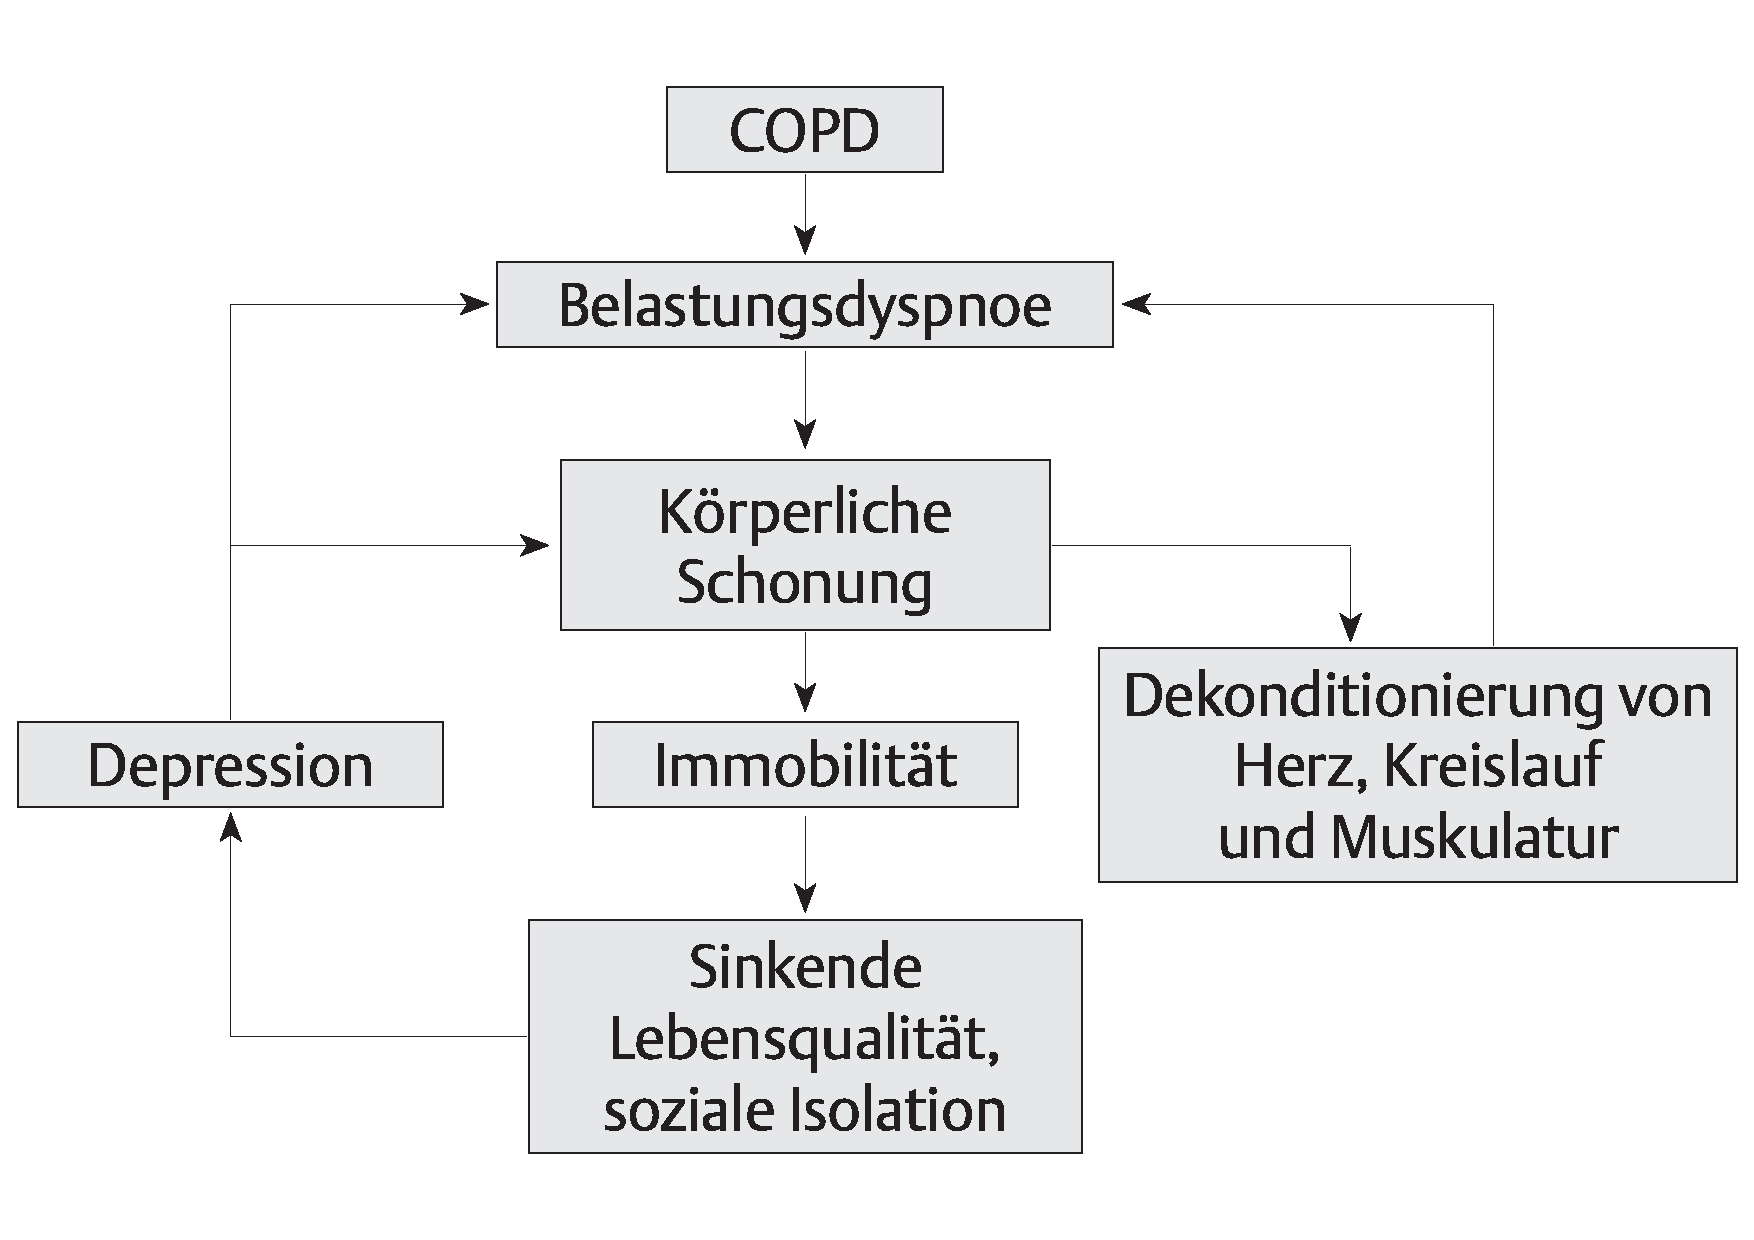
\includegraphics[width=0.6\textwidth]{teufelskreis}
  \caption{Circulus virtuosus, übernommen aus \cite[e19]{vogelmeier2007}}
  \label{fig:copd_teufelskreis}
\end{figure}

Die Angaben zur Prävalenz von Angst und Depression bei COPD variieren sehr. „Generalisierte Angststörungen werden in einer Häufigkeit von 2-16\%, Panikstörungen von 8-67\%, depressive Symptome und Depressionen zwischen 11 und 80\% sowie Angstsymptome in einem Bereich von 10-75\% angegeben“  \autocite[34]{kenn2011}.

An diesen Zahlen lässt sich erkennen, dass exakte Ergebnisse in Bezug auf die Prävalenz noch fehlen. Kenn und Kühl gehen davon aus, dass methodisch verschiedene Diagnoseansätze hierfür verantwortlich sind, wobei sie hierbei Ergebnisse aus Interviews, die sich an den Kriterien für psychische Störungen z.B. nach der ICD 10 orientieren, und Fragebögen gegenüberstellen. Generell erschwerten wohl neben den unterschiedlichen Erhebungsinstrumenten auch die Heterogenität der untersuchten Patientenkohorte mit verschiedenen Schweregraden die Interpretation der Ergebnisse \autocite[vgl.][35]{kenn2011}.
Zudem geben die Studienergebnisse keine Auskunft darüber, in wie weit bei Patienten, die eine COPD aufgrund eines längeren Nikotinabusus‘ entwickelt haben, bereits eine größere psychische Vulnerabilität und somit ein erhöhtes Risiko für die Ausbildung einer Depression oder Angst-/Panikstörung besteht. 

Ein evtl. wichtiges Konzept für den Krankheitsverlauf der COPD in seinen unterschiedlichen Facetten scheint die s.g. „Fear Avoidance" zu sein. Viele Patienten berichten von Angst vor auftretender Atemnot. Fear Avoidance- Konzept meint „die Angst vor der Verstärkung eines Krankheitssymptoms bzw. Verschlechterung des Verlaufs und daraus folgende Aktivitätsvermeidung" \autocite[111]{stenzel2013}. Dieses Konzept wurde jedoch bisher für COPD noch kaum diskutiert und erforscht. Eine neuere Studie zeigte jedoch, dass Fear Avoidance tatsächlich als Mediator des Zusammenhangs zwischen COPD-Status und Lebensqualität bzw. Gesundheitsstatus gesehen werden kann. Die Autoren plädieren daher dafür, dass im Rahmen der pneumologischen Rehabilitation auch psychotherapeutische Interventionen implementiert werden sollten, welche diesen Aspekt aufgreifen \autocite[112]{stenzel2013}. 

In dem später dargestellten musiktherapeutischen Konzept wird dieser Aspekt ebenfalls implizit aufgenommen werden. Durch achtsames Wahrnehmen eigener Grenzen und Möglichkeiten, aber auch durch übungszentriertes Arbeiten entwickeln die Patienten durch positive Erfahrungen im Zusammenhang mit Selbstregulation wieder mehr Selbstvertrauen und erleben sich als selbstwirksame Individuen, die sich nicht der auftretenden Atemnot ausgeliefert fühlen müssen.

In Studien wurde zudem ein signifikanter Zusammenhang zwischen einer erhöhten Mortalität und einer COPD mit begleitender depressiver oder Angstsymptomatik nachgewiesen. Aber auch in Bezug auf die Exazerbations- und Rehospitalisationsrate sowie die Leistungsfähigkeit und -bereitschaft von COPD-Patienten scheint hier die Ausbildung der genannten psychischen Erkrankung einen relevanten negativen Faktor darzustellen\autocite[vgl.]{kenn2011}.

Obgleich das zuvor Erläuterte heutzutage unter allgemeinmedizinischen und pneumologischen Fachärzten als bekannt anzunehmen ist, wird die Problematik in den Arzt-Patient-Gesprächen oftmals nicht thematisiert. Eine amerikanische Studie zeigte diese Diskrepanz zwischen der Prävalenz und Behandlungshäufigkeit psychischer Erkrankungen bei gleichzeitiger COPD. In einer Telefonumfrage von 1334 Patienten lagen bei 61\% psychische Auffälligkeiten, insbesondere Angstsymptome, vor. Lediglich 31\% dieser Patienten wurden diesbezüglich behandelt \autocite[vgl.][156]{fischer2007}.


\section{Zusammenfassende Betrachtung}
\label{zusammenfassende betrachtung}
Die vorherigen Ausführungen machen deutlich, um welch komplexes und schwerwiegendes Krankheitsbild es sich bei der COPD handelt. 

% ---------------------------------------------------------------------------
% ----------------------- end of thesis sub-document ------------------------
\newpage\thispagestyle{empty}
% this file is called up by thesis.tex
% content in this file will be fed into the main document

%: ----------------------- introduction file header -----------------------
\chapter{Musiktherapeutische Stimmarbeit}
\label{chapter:musiktherapeutische_stimmarbeit}
\setlength{\epigraphwidth}{8.0cm}
\epigraph{Singen als Ausdruck von Gefühl, Gedanken und Identität, als Bewältigung und soziale Aktivität, die Fühlen und Denken synchronisiert und Gemeinschaftsgefühl, Nähe und Zugehörigkeitsgefühl erzeugt, ist ein Kommunikationsmedium, das von frühester Kindheit bis in die letzten Lebensphasen des Menschen eine besondere Rolle spielt.}{Heiner Gembris} todo Fußnote Gembris 2008 S. 12
\ifpdf
    \graphicspath{{3_musiktherapeutische_stimmarbeit/figures/PNG/}{3_musiktherapeutische_stimmarbeit/figures/PDF/}{3_musiktherapeutische_stimmarbeit/figures/}}
\else
    \graphicspath{{3_musiktherapeutische_stimmarbeit/figures/EPS/}{3_musiktherapeutische_stimmarbeit/figures/}}
\fi
% ----------------------------------------------------------------------
%: ----------------------- introduction content -----------------------
% ----------------------------------------------------------------------
\lettrine{I}{n} diesem Zitat wird in knapper, jedoch prägnanter Form zusammengefasst, wie wichtig und wertvoll der stimmliche Ausdruck für den Menschen ist. In den folgenden Kapiteln soll das hier Skizzierte ausgeführt und -geweitet werden, um einen Eindruck für die Möglichkeiten der Stimmarbeit im musiktherapeutischen Kontext zu vermitteln.

Bevor im Folgenden selbstverständlich mit dem Begriff der "Stimme" umgegangen wird, scheint es sinnvoll, eine kleine Einführung in die Physiologie des Stimmapparats zu geben, um zum Einen die Komplexität der Funktionsweise unseres körpereigenen Instruments zu verstehen und um zum Anderen eine gemeinsame Grundlage für die Ausführungen in den nun folgenden Kapiteln zu schaffen. 

Die Stimmerzeugung basiert auf dem Zusammenspiel zwischen Körper, Atem und Stimmapparat (Kehlkopf und Ansatzrohr). Atem und Kehlkopffunktionen sind abhängig von dem Zusammenspiel und dem Spannungszustand der Muskeln. Haben wir beispielsweise aufgrund eines plötzlich auftretenden angstauslösenden Ereignisses einen erhöhten Körpertonus, so wird dies zwangsweise dazu führen, dass wir nicht mehr entspannt ein- und ausatmen, da sich die erhöhte Anspannung auch auf unsere Atemmuskulatur, insbesondere dem Zwerchfell als wichtigstem und größtem Atemmuskel überträgt. 

Für die Stimmerzeugung sind verschiedene Faktoren wichtig, die jedoch nicht einzeln nebeneinander stehen, sondern vielmehr ineinander übergreifen. 

Bevor es zu einer stimmlichen Äußerung kommt, bedarf es des Einfließens der Luft in die unteren Atemwege, die Lunge. Die Atmung als lebensnotwendiger Prozess wird über das Vegetativum gesteuert, das heißt, sie erfolgt nicht willentlich gelenkt; auf die Atmung im Speziellen wird unter Kapitel 3.2.5 näher eingegangen. Die Atemluft strömt für normal durch die sich im Kehlkopf befindenden und in Dreicksform geöffneten Stimmlippen. Kommt es nun zu einer stimmlichen Äußerung, schließt sich im ersten Schritt die Glottis, auch Stimmritze genannt, nach vollendetem Einatmen. Anschließend wird durch den nun folgenden Ausatem ein Überdruck auf die geschloßenen Stimmlippen erzeugt, welcher diese in Schwingung versetzt.
Für die Stimmerzeugung nun bedarf es des Ausatemstroms, welcher einen Überdruck erzeugt, der wiederum auf die Glottis, die s.g. Stimmritze, wirkt und sie kraftvoll öffnet. 
Stimmphysiologische Hintergründe todo

In den folgenden Kapiteln wird 

\section{Geschichtliche Einführung in das Thema}
Zu Beginn der weiteren Ausführungen in diesem Kapitel sollte der Blick auf den Gebrauch der Singstimme in der Gesellschaft gewendet werden, um ein klareres Gesamtbild dieses Themas entstehen lassen zu können.

Während das Singen in unserer Großelterngeneration noch weit verbreitet war, man beachte unseren großen Umfang an deutschem Liedgut, so hat die nationalsozialistisch geprägte Zeit der 30er und 40er Jahre einen Keil in diesen selbstverständlichen Gebrauch der Singstimme in Gemeinschaft getrieben.
Die Verschandelung deutschen Liedguts mit nationalsozialistischem Gedankengut und den Einsatz desgleichen für propagandistische Zwecke, sowie im Besonderen in der Jugendmusikbewegung der damaligen Zeit geschehen, führte u.a. zu "der späteren Voreingenommenheit gegenüber gemeinsamem Singen im Allgemeinen und gegenüber dem deutschen Volkslied im Speziellen" \autocite[9]{wolf2012}.

Hinzu kommt seitdem die Entwicklung neuer Medien und die Möglichkeit eines geöffneten Zugangs zu diesen. Laut Wolf hat dies großen Einfluss auf "die Entwicklung hin zu einer Vereinzelung der Menschen und hin zu einer Veränderung des menschlichen Alltagverhaltens" \autocite[10]{wolf2012}, wodurch die Notwendigkeit der gemeinschaftlichen Freizeitgestaltung, welche in früheren Zeiten oftmals das gemeinsame Singen beinhaltete, nachließ. Nur an vereinzelten Schauplätzen wie z.B. im Gottesdienst, im Stadion, bei den Pfadfindern oder in Chören wird das gemeinschaftliche Singen und/oder Grölen noch aktiv praktiziert.

In der MT war der Einsatz der Singstimme ebenfalls lange Zeit negativ konnotiert und wurde "[\ldots] als "Konflikt vermeidende Technik" in den heilpädagogisch orientierten Bereich der Kindermusiktherapie oder das palliativ orientierte Feld der Geriatrie verortet" \autocite[10]{wolf2012}. So war das Singen von Liedern im Rahmen einer "psychotherapeutisch orientierten MT" lange Zeit ausgeklammert. Zudem wurde die Stimme zum klanglichen Ausdruck kaum genutzt, da man einen zu großen Widerstand seitens der Patienten erwartete (siehe weiter unten in diesem Kapitel). 

Durch den sich in den letzten Jahren vollziehenden Paradigmenwechsel in der psychotherapeutischen Behandlung im Allgemeinen und der musiktherapeutischen im Speziellen von einem eher konfliktzentrierten Ansatz und dem Konzept der Katharsis hin zu einem eher ressourcenorientierten und stabilisierenden Arbeiten veränderte sich auch die Einstellung gegenüber dem Singen\autocite[vgl.][11]{wolf2012}. Einer kleinen Forschergruppe aus Musiktherapeuten und -pädagogen, aber auch bekannten Ärzten (wie z.B. Dr. Gerald Hüther, Dr. Manfred Spitzer u.a.) ist es zu verdanken, dass wir heute mehr über die Wirkung des Singens auf Körper, Geist und Seele wissen. Sie waren es, die zu einer Etablierung von Singgruppenarbeit primär beigetragen haben. Im klinischen Bereich hat sich insbesondere der Musiktherapeut Wolfgang Bossinger verdient gemacht und eine mittlerweile über Deutschland verbreitete Initiative, "Singende Krankenhäuser", ins Leben gerufen. Aber auch Sabine Rittner und Karl Adamek haben zu einem großen Erkenntnisgewinn und möglichen Vorgehensweisen in diesem Bereich verholfen.

\section{Einsatz der (Sing-)Stimme im musiktherapeutischen Kontext}

Heute wird die (Sing-)Stimme im psychotherapeutischen Kontext in unterschiedlicher Art und Weise eingesetzt, genutzt und betrachtet. Sabine Rittner \autocite[vgl.][204 ff.]{rittner2008} hat diese Bereiche kategorisiert, um ihre Komplexität zu entzerren. Diese insgesamt acht Kategorien fließen zum Teil in die folgenden Ausführungen ein: 
Stimme als\ldots
\begin{enumerate}
\item Medium der verbalen und nonverbalen Beziehungsgestaltung
\item Methode in der körperorientierten Musikpsychotherapie
\item Diagnostikum im therapeutischen Gespräch
\item Indikator für die therapeutische Übertragung- und Gegenübertragung
\item Symptom
\item Ausdrucksmittel
\item Selbstheilungs-Mittel
\item Medium zur Tranceinduktion
\end{enumerate}

Bereits im Mutterleib beginnt der Beziehungsaufbau zwischen Mutter und Kind über stimmliche Äußerung. Ab der 23. Schwangerschaftswoche kann der Fötus seine Umwelt auditiv wahrnehmen und auf sie reagieren. Die Stimme der Mutter tritt dabei in den Vordergrund. Wie man durch Untersuchungen kurz nach der Geburt festgestellt hat, können Säuglinge die Stimme ihrer Mutter von der anderer Personen unterscheiden \autocite [vgl.][22f]{noecker-ribeaupierre2004}. 

Die stimmliche Äußerung ist für die Entwicklung des Kindes von besonderer Bedeutung: durch Abstimmungsprozesse mit den primären Bezugspersonen auf unterschiedlichen sensorischen Ebenen, insbesondere durch stimmliche Interaktion, lernt es, die Welt und sich über die s.g. amodale Wahrnehmung zu begreifen. Gerade in dieser Zeit wird deutlich, welche Bedeutung die Stimme im Hinblick auf die Mitteilung der eigenen emotionalen Gestimmtheit hat, wie sich Beziehung ohne Worte aber dennoch durch stimmlichen Ausdruck gestalten lässt. Insbesondere durch den Einsatz von Vokalen kann diese "emotionale Tönung" \autocite[205]{rittner2008} deutlich werden, wie weiter unten näher erläutert wird.

Rittner \autocite [vgl.][106f.]{rittner1990} betont zudem die therapeutische Relevanz der Polaritäten, die sich im Schreien und Lallen des Säuglings äußern. Mit dem ersten Schrei tritt der Säugling zum ersten Mal geräuschvoll mit seiner neuen/ alten Umwelt in Kontakt und entlädt dabei die zuvor im ersten Einatem aufgebaute Anspannung. Diese Form der Kontaktaufnahme mit der Außenwelt differenziere sich, so Rittner, in den darauffolgenden Wochen immer mehr zu einem "gerichteten Appell" in Bezug auf die Befriedigung der Grundbedürfnisse. Im Lallen hingegen zeige der Säugling aus einer befriedigten Grundstimmung heraus eine "lustbetonte, nach innen gerichtete, autoerotisch-regressive Handlung", die oftmals unterbrochen wird, sobald beispielsweise im Außen Geräusche auftreten oder eine Person das Zimmer betritt und ihn so aus seiner Versunkenheit herauszieht. 
Die o.g. Polaritäten können aus diesen beiden Handlungen heraus folgendermaßen beschrieben werden: "die Verbindung zwischen Innenraum und Außenraum, zwischen Regression, dem wohligen Sich-Einhüllen, und Progression, in der sich lebenserhaltende aggressive Anteile artikulieren" \autocite[vgl.][106f.]{rittner1990}.

Diese Aspekte sind wesentlich für die Gestaltung und die Arbeit im Rahmen einer therapeutischen Beziehung. Mithilfe musiktherapeutischer Stimmarbeit ist es uns somit möglich, in sehr direkter Form an diese sehr frühen Erfahrungswelten anzuknüpfen und an einer Ausbalancierung der o.g. Polaritäten zu arbeiten. 

Allerdings gilt es dabei u.a. zu beachten, dass der Mensch im Laufe seiner Entwicklung Hemmungsmechanismen ausbildet, welche auf die Sauberkeitserziehung sowie auf Sozialisationsprozesse zurückzuführen sind. Diese Mechanismen lassen sich gliedern in "Scham- und Peinlichkeitsgefühle als auch [in] psychische Instanzen, die das Gewissen und Schuldgefühle auslösen" \autocite [106f.]{rittner1990}. 

Durch das Singen kommen wir, wie bereits zuvor dargelegt, schnell in Kontakt mit unserer primär unbewussten Gefühlswelt. Aufgrund der Nähe zu "frühkindlichen Gefühlszuständen vor der Schamhemmung" (todo Klausmeier zitiert in Rittner 1990 todo) und damit einem sehr intensiven emotionalen Erleben kann der unvorbereitete Einsatz der Singstimme überflutend und angstauslösend hinsichtlich des ungewollten Zeigens von u.a. abgewehrten Selbstanteilen wirken. 

Da das Thema Scham m.E. wichtig ist für die Arbeit mit der Stimme im musiktherapeutischen Rahmen und bereits am Anfang dieses Kapitels in Wolfs Aussage zu Widerständen in diesem Kontext anklingt, soll an dieser Stelle darauf eingegangen werden.

\subsection{Scham und Stimme}
Zunächst eine kurze Erläuterung des Begriffs. Unter dem Titel "Scham. Lautloses Tönen" erschien 2012 ein Themenheft der Musiktherapeutischen Umschau (MU). Hierin beschrieb Tilman Weber in knapper Form und aus unterschiedlichen theoretischen Perspektiven die "Scham" folgendermaßen:
"Vielleicht kann man sagen, dass Scham aus triebpsychologischer Sicht einem typischen Es - Überich - Konflikt entspringt, aus objektpsychologischer Sicht der Diskrepanz zwischen Individuum und Gesellschaft und aus ichpsychologischer Sicht der Differenz zwischen Anspruch und Vermögen" \autocite[215]{weber2012}. 

Tiedemann, tiefenpsychologischer und analytischer Psychotherapeut und Forscher, beschreibt Scham als einen Vorgang, in dem "das Subjekt eine Infragestellung und Bedrohung der sozialen Wertschätzung, Akzeptanz und Anerkennung" \autocite[219]{tiedemann2012} erlebt. Daher tritt sie meist in solchen Situationen auf, in denen ein "Mensch etwas Intimes preisgibt" \autocite[219]{tiedemann2012}. 

Die Stimme ist das intimste körpereigene Instrument des Menschen. Jede stimmliche Äußerung gibt ein Stück unserer individuellen Ge-stimmt-heit preis. An unterschiedlichen Stellen in der hierzu relevanten Literatur wurde immer wieder darauf hingewiesen, dass eine stimmliche Maskierung des eigenen affektiven Zustandes nicht möglich ist \autocite[vgl.][279]{decker-voigt1992} \autocite[vgl.][481]{rittner2009a}. Je nach Stellung der Stimmknörpelchen und des Tonus der über 100 an der stimmlichen Äußerung beteiligten Muskeln \autocite[vgl.][40]{cramer1998} gestaltet sich das nach außen Dringende. Denn jegliches Zurückhalten oder Verdecken von aufkeimenden Emotionen führt zu Störungen der Feinabstimmung innerhalb des Stimmapparates. Dies kann zu Muskelverspannungen führen, die wiederum in der erklingenden Stimme durch einen harten Stimmansatz, verhauchen der Stimme durch nicht zu Klang gewordener herausströmender Luft, eine höhere oder tiefere Stimmfrequenz u.a. zu hören sind \autocite[vgl.][279]{decker-voigt1992}. 
Laut Rittner vernehmen wir die "emotionale Tönung" der Person durch die Prosodie [=das, was dazu singt). Insbesondere durch den Klang der Vokale, welche physikalisch betrachtet als Klangträger gleichmäßige Schwingungsmuster, Konsonanten hingegen als Geräuschträger ungleichmäßige Schwingungswellen erzeugen, erfahren wir im Sinne der oben genannten physiologischen Vorgänge etwas über die Gestimmtheit unseres Gegenübers. Dabei kommt dem Singen eine besondere Rolle zu: "Singen unterscheidet sich vom Sprechen dadurch, dass der klanglich-nonverbale Schwingungsanteil der emotionalen Botschaft durch die Verlängerung der Vokale im ausgedehnten Ausatem deutlich in den Vordergrund tritt" \autocite[205]{rittner2008}.

Die vorherigen Ausführungen machen deutlich, dass es sich bei der gesanglichen Äußerung um ein sehr unmittelbares und intimes Zeigen der emotionalen Verfassung handelt. Die stimmliche Äußerung ist direkter als das Spielen eines Musikinstruments, welches bereits räumlich von uns getrennt ist und evtl. sogar einen Schutz bietet i.S. eines sich dahinter Verstecken-Könnens. Wenn wir also im musiktherapeutischen Kontext mit der Singstimme arbeiten, sollten wir uns dieser unmittelbaren Verbindung bewusst sein. Denn das Singen, vorallem in der Improvisation, welche häufig mit der Sorge um Kontrollverlust verbunden ist, kann als "zu starker emotionaler Ausdruck abgewehrt und blockiert werden" \autocite[485]{rittner2009a}. Um jedoch der Abwehr aus Scham entgegen zu wirken, sei es laut Rittner wichtig, stimmliche Interventionen im Verlauf der musiktherapeutischen Behandlung methodisch anzubahnen. So könne beispielsweise mit bekannten, durchkomponierten Liedern, Melodien und Rhythmen begonnen werden, um sich der ursprünglichen stimmlichen, improvisierenden Äußerung, wie sie zu Beginn des Lebens wertfrei bestand, zu nähern. 

\subsection{Diagnostische Überlegungen}
Im Rahmen der Diagnostik gibt die Stimme des Patienten bereits wichtige Hinweise auf dessen aktuelle Befindlichkeit sowie seine Stimmung. Durch aufmerksames Hinhören kann erspürt werden, ob das Gesagte in sich "stimmig", sprich kongruent ist. Zudem gibt sie bereits Auskunft über den biografischen Hintergrund der sich äußernden Person, denn sie hat sich mit unseren über die Zeit gesammelten Lebenserfahrungen weiterentwickelt und diese in sich aufgesogen. So gilt die Stimme unter Experten als "Klingendes Hologramm der Persönlichkeit" \autocite{adamek1999}, "lauthafte Biographie" \autocite{gundermann1994} und bei Rittner erfahren wir über den Klang der Stimme etwas über die "leib-seelische Gewordenheit" \autocite[211]{rittner2008} des Menschen.
Dabei scheint jedoch nicht so sehr der Inhalt des Gesagten aufschlussreich, sondern vielmehr der "Klang der Stimme (Klangspektrum, Modulation, Lautstärkeänderungen, Stimmsitz, Vokaleinsatz etc.), die Sprechweise (Artikulation, Phrasierung, Pausensetzung etc.) und die Atmung (Atemfrequenz, Atemtiefe, hörbares Einatmen, Sitz des Atemraumes im Körper etc.)" als auch "die Art der Gestaltung von Sprechpausen, Abbrüchen, Momenten des Innehaltens, Verzögerungen u.ä." \autocite[210]{rittner2008}. Diese stillen Momente vertiefen jedoch oftmals das atmosphärische Wahrnehmen und können zu einem tieferen Verstehen ohne Ablenkung führen. 
Gerade in Momenten der Inkongruenz von Semantik, Prosodie, Mimik, Gestik etc. wurde festgestellt, dass der Zuhörer sich in diesem Falle weniger auf den Inhalt des Gesprochenen seines Gegenübers bezieht, sondern in einen visuell-auditiven Modus wechselt, in welchem die Semantik in den Hintergrund rückt \autocite [vgl.][206f.]{rittner2008}.

\subsection{Weitere Aspekte musiktherapeutischen Arbeitens mit der Stimme}
Rittner

\subsection{Vokalimprovisation}
Die Vokalimprovisation ist eine sehr spielerische Möglichkeit, die Stimme in die musiktherapeutische Arbeit einzubeziehen. Sie gilt als der "Einsatz des gesamten Ausdrucksspektrums stimmhafter wie stimmloser Äußerungen, meist im Schutz einer Gruppe mit oder ohne Themenvorgabe" \autocite [108]{rittner1990}. Dabei sei sie stets gebunden an persönliche, situative, musikalisch oder symbolische Inhalte und verfolge therapeutische, pädagogische oder musikalisch-künstlerische Ziele \autocite [109]{rittner1990}.


\subsection{Die Wichtigkeit des Einbezugs von Körper und Atem in dieser Arbeitsweise}
Ilse Middendorf
Schlaffhorst Andersen
MT und Atem (Buch)
Annette Cramer
Rittner
Hertha Richter

\section{Die Wirkung des Singens auf Körper und Psyche} 
Bossinger, Adamek und Cramer
Selbstheilungskräfte





\newpage\thispagestyle{empty}
% ----------------------------------------------------------------------
\ifpdf
    \graphicspath{{4_konzept/figures/PNG/}{4_konzept/figures/PDF/}{4_konzept/figures/}}
\else
    \graphicspath{{4_konzept/figures/EPS/}{4_konzept/figures/}}
\fi

%: ----------------------- introduction file header -----------------------
\chapter{Konzeptionelle \"Uberlegungen}
\label{chapter:konzeptionelle_ueberlegungen}
Die vorangegangenen Auseinandersetzungen mit den Themen COPD und Musiktherapeutische Stimmarbeit dienten dem Aufbau einer Basis, um nun auf dieser ein eigenes Konzept entwickeln zu können. 

Dieses Konzept für die musiktherapeutische Stimmarbeit mit COPD-Patienten ist als übungs- und erlebniszentriertes sowie ressourcenorientiertes Gruppenverfahren angelegt, welches auf der Grundlage psychodynamisch orientierter Musiktherapie Aspekte aus der Körper- und Atemarbeit, Achtsamkeitslenkung und Stimmbildung mit einbezieht. Die folgenden Abschnitte sollen dies nun weiter ausführen und erklären. Am Ende des Kapitels wird ein beispielhafter Sitzungsaufbau beschrieben. Um für die Praxis gut vorbereitet zu sein, wurden im Verlauf des Masterarbeits-Prozesses verschiedene, als geeignet erscheinende Übungen gesammelt, welche in Form einer Literaturliste dem Anhang beigefügt sind.

Im Verlauf der Auseinandersetzung mit diesem Masterarbeitsthema wurden in Fort- und Weiterbildungen (Singende Krankenhäuser, ein atemtherapeutisches Seminar bei Matthias Grot, Wochenendseminare bei Astrid Schmid zur Methode "`Atem-Tonus-Ton"') sowie Selbsterfahrungsseminaren etliche Übungen und Ideen für die praktische Arbeit gesammelt. Da die schriftliche Ausführung dieser Sammlung jedoch den Rahmen dieser Arbeit sprengen würde, wurde dem Anhang eine Liste geeigneter Literatur zu diesem Thema beigefügt.

\section{Psychodynamische \"Uberlegungen}
\label{psychodynamische_ueberlegungen}
In Kapitel \ref{chapter:copd} wurde bereits dargelegt, dass die Diagnose einer COPD auch auf psychischer Ebene für Patienten mit Veränderungen hinsichtlich der möglichen Ausbildung psychischer Komorbiditäten verbunden sein kann. In welchem Ausmaß dies geschieht und mit welchen Folgen es verbunden sein kann, ist individuell abhängig von den jeweiligen biographischen Hintergründen und den damit verbundenen Entwicklungsmöglichkeiten hinsichtlich einer stabilen, gefestigten psychischen Verfassung sowie mit einem unterstützenden sozialen Umfeld.

Wie bereits unter 2. näher erläutert, wird eine COPD nur unter bestimmten Umständen ausgebildet: genetische Veranlagung, Umweltverschmutzung und Einatmen von Schadstoffen bspw. im beruflichen Umfeld sowie zum größten Teil durch einen länger andauernden Nikotin-Abusus (betrifft ca. 80\% der Patienten). 

Was bedeutet aber letzteres nun für die therapeutische Behandlung dieser Patienten? Meines Erachtens scheint es wichtig, diese Suchtthematik mitzudenken und aufzugreifen, da damit suchtspezifische psychische Aspekte verbunden sind. Diese bringen Besonderheiten insbesondere in der Gegenübertragung mit sich bringen, wodurch die Auseinandersetzung mit diesem Thema seitens des Therapeuten für die Behandlung abhängiger Patienten unumgänglich erscheint. Es ist mir natürlich bewusst, dass mit dieser Erklärung nicht alle potentiellen Patienten eingeschlossen sein werden, aber aufgrund der hohen Relevanz der Nikotinabhängigkeit in Verbindung mit der Ausbildung einer COPD bedarf es eines Einbezugs dieser Problematik in therapeutische Konzepte. Es gilt natürlich in der Praxis diese Annahmen stets zu überprüfen und bei Bedarf anzupassen bzw. individuell zu verändern.

Bevor jedoch auf spezielle psychodynamische Aspekte eingegangen wird, bedarf es einer kurzen definitorischen Erläuterung, was unter dem Phänomen Sucht im deskriptiven Sinne verstanden werden kann. 

\begin{quote}
\onehalfspacing
"`Das süchtige Verhalten besteht in dem anhaltenden, starken, unwiderstehlichen Drang, bestimmt durch Drogen bzw. andere Substanzen oder auch durch Tätigkeiten [...] hervorgerufene innere Zustände und Befindlichkeiten von Entspannung oder Anregung immer wieder aufzusuchen oder herbeizuführen."' \autocite[173]{mentzos2011} 
\end{quote}

Betroffene tendieren dazu, im Verlauf die Suchtmittel-Dosis immer mehr zu erhöhen. So sind die Übergänge zwischen normalem Gebrauch und Missbrauch des Suchtmittels bis zur psychischen und körperlichen Abhängigkeit fließend \autocite[vgl.][173]{mentzos2011}. Im ICD-10 findet sich das Störungsbild der Tabakabhängigkeit unter F17 im Bereich der psychischen Störungen; auch das DSM-IV beschreibt das Störungsbild in ihrem Diagnostischen und Statistischen Manual Psychischer Störungen. Um eine Abhängigkeit diagnostizieren zu können, müssen mindestens drei von insgesamt sechs im ICD-10 beschriebenen Kriterien seit 12 Monaten vorherrschen. Diese umfassen:

\begin{itemize}
\item "`starkes Verlangen oder eine Art Zwang, Substanzen oder Alkohol zu konsumieren
\item verminderte Kontrollfähigkeit
\item körperliches Entzugssyndrom
\item Toleranzentwicklung (Dosissteigerung)
\item Vernachlässigung anderer Interessen
\item anhaltender Substanz- oder Alkoholkonsum trotz Nachweis schädlicher Folgen (körperlich, psychisch sozial)"' \autocite[315]{moeller2009}
\end{itemize}

Für die Entstehung und Aufrechterhaltung der Sucht dürfen natürlich die neurobiologischen Prozesse nicht außer Acht gelassen werden. Es wird davon ausgegangen, dass "`es sich bei der stoffgebundenen Sucht um die neurochemische Anpassung des Gehirns an eine anhaltende Substanzzufuhr"' \autocite[14]{tretter2008} handelt. Den Antrieb für das süchtige Verhalten bildet ein neurochemisch begründbarer Belohnungseffekt des Suchtstoffes. Dieser Aspekt ist m.E. selbst aus psychodynamischer Sicht wichtig, da es hier vermutlich zu einem Wechselspiel dieser unterschiedlichen Faktoren kommt und sich aus einer vormals psychischen Abhängigkeit oftmals eine körperliche entwickeln kann.
Darüber hinaus bestehen in Bezug auf die Hintergründe der Suchtentwicklung noch weitere theoretische Modelle (Verhaltenstherapie, Stress-Konzept u.a.) \autocite[vgl.][38ff.]{tretter2008}, auf welche jedoch an dieser Stelle nicht weiter eingegangen werden kann.
 
Folgt man psychoanalytischen Theorien zur Suchtentwicklung, kann davon ausgegangen werden, dass bei Menschen mit einer ausgeprägten Suchtproblematik in der frühen Kindheit ein wichtiger Erfahrungsbereich nicht ausreichend genährt wurde (\cite{mentzos2011}, \cite{weidlinger2012} und \cite{ermann1999}): ein Gefühl für die eigenen Bedürfnisse ist nicht ausreichend entwickelt, wodurch auch das Erkennen der Wichtigkeit des sich dafür Einsetzens für diese sowie die eigenverantwortliche Umsetzung entsprechender Handlungen erschwert ist. Dafür bedarf es der frühen Erfahrung, dass ein Kind im Außen diese auf sich bezogene und abgestimmte Zuwendung und Wertschätzung erfahren hat. Austauschprozesse zwischen dem Kind (dem Selbst) und dem Anderen (dem Objekt) im zuvor genannten Sinne, wodurch das heranwachsende Kind "`gute"' Objekte internalisieren kann, sind essentiell für die Entwicklung einer stabilen Persönlichkeit. Dieses Postulat entspringt primär der Objektbeziehungstheorie im Sinne Melanie Kleins. In Bezug auf die Suchterkrankung wird hier davon ausgegangen, dass es sich immer um eine Beziehungskrankheit handelt, welche vermutlich ihren Ursprung in der frühen Kindheit im Übergang von der Symbiose zur Individuation hat \autocite[vgl.][9]{weidlinger2012}. Kann das Kind aufgrund wiederholter Ablehnung, mangelhafter Feinfühligkeit oder gar wegen an ihm ausgeübter körperlicher oder seelischer Gewalt kaum positive Selbstobjekte ausbilden, treten an deren Stelle negative Selbstobjekte. So wird das Kind vermutlich im weiteren Verlauf innerlich mit ambivalenten, polarisierenden Gefühlen sowie mit der Schonung oder aggressiver Wut auf die Objekte beschäftigt sein\autocite[vgl.][10]{weidlinger2012}. 

Diese Ambivalenz zeigt sich ebenfalls in der Sucht, da das Suchtmittel als Beziehungsobjekt sehr ambivalent besetzt ist. "`Auf der einen Seite wirkt es tröstend, beruhigend, entängstigend oder berauschend und anregend; auf der anderen Seite aber bringt es dem Süchtigen Leid, Schuldgefühle, körperliche und seelische Zerstörung bis hin zum Tod"' \autocite[175]{mentzos2011}. Jedoch zeigt sich hierin m.E. primär die "`verinnerlichte Tendenz zur Selbstabwertung wie Selbstzerstörung"' \autocite[10]{weidlinger2012}. Dieser Aspekt, des mangelnden Selbstwertgefühls aufgrund einer strukturellen Störung, findet sich in den psychodynamischen Theorien der Sucht immer wieder vor. 

So wie beispielsweise in der Sucht-Theorie der Selbst-Psychologie nach Kohut, wird dem Suchtmittelkonsum die Funktion einer Ersatzbefriedigung hinsichtlich mangelhaft genährter narzisstischer Bedürfnisse zugeordnet. Auch Mentzos (2011) schreibt, dass "`das Suchtmittel(...) zum Mittel der notdürftigen Kompensation einer gestörten Selbstwertgefühlregulation"' werde, somit als Ersatz für ein stützendes narzisstisches Selbstobjekt dient. So kann das Suchtverhalten auch als Versuch des Betroffenen verstanden werden, die eigene, innere Sicherheit mithilfe des Suchtmittels wieder herzustellen, welche zuvor durch Enttäuschungen, Kränkungen, Vernachlässigung oder tiefgreifende Konflikte verloren gegangen war. Tress zufolge handelt es sich bei der Sucht um einen Versuch der "`Selbstheilung"'(\cite{tress1985} zitiert in \cite[222]{ermann1999})

Folgt man diesen vorherigen Überlegungen, so kann davon ausgegangen werden, dass bei Menschen mit einer entwickelten Suchtproblematik eine erhöhte Vulnerabilität in Bezug auf ihr Selbstempfinden besteht. Dieser Aspekt könnte meines Erachtens in Bezug auf die Krankheitsbewältigung einer ausgebildeten COPD wichtig sein, wie im Folgenden näher erläutert wird.

Bei Daniel Stern finden sich sehr essentielle Vorstellungen für die Entwicklung eines Selbstempfindens wieder. Diese sind jedoch nicht nur in Bezug auf die kindliche Entwicklung von großer Wichtigkeit, sondern bleiben es für das gesamte Leben. Stern unterscheidet hierbei zwischen sechs verschiedenen Bereichen, welche letztlich das Selbst des Menschen bilden: das auftauchende Selbst, das Kern-Selbst, das intersubjektive Selbst, das verbale Selbst sowie mittlerweile das narrative Selbst. Dabei gliedert er seit ein paar Jahren die Empfindung eines Kern-Selbst in zwei Bereiche: zum Einen in die Empfindung eines Kern-Selbst mit seinen drei Invarianzen von Urheberschaft, Kohärenz und Kontinuität und zum Anderen in die Empfindung eines Kern-Selbst in Gemeinschaft mit dem Anderen.  Wie in der Grafik ersichtlich wird, haben die ersten 3 Bereiche nach Sterns neueren Erkenntnissen ihren Ursprung bereits in der pränatalen Phase. \footnote{Da an dieser Stelle nicht auf alle Bereiche des Selbstempfindens ausführlich eingegangen werden kann, empfiehlt sich ein Blick in Daniel Sterns Werk "`Die Lebenserfahrung des Säuglings"', in welchem der Entwicklungspsychologe, Säuglingsforscher und Psychoanalytiker in sehr anschaulicher Weise die Entwicklung des Säuglings anhand der Entwicklung eines umfassenden Selbstempfindens erläutert.}


\begin{figure}
 \centering
  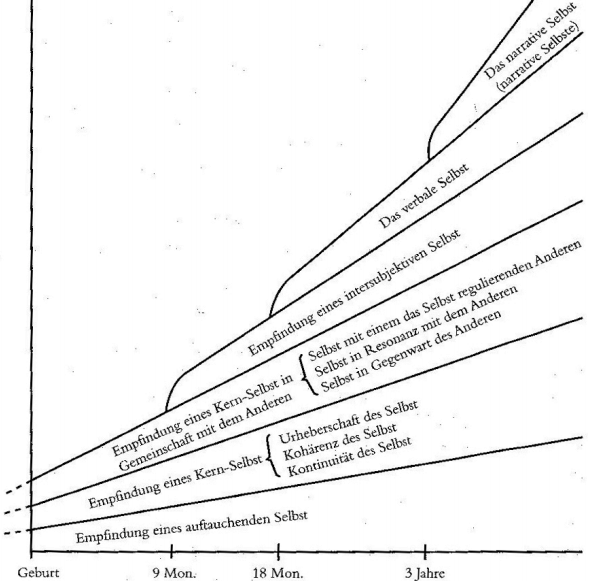
\includegraphics[width=0.7\textwidth]{selbstempfindungen}
  \caption{Die sechs Selbstempfindungen nach Daniel Stern}
  \label{fig:selbstempfindungen}
\end{figure}


In Bezug auf eine entwickelte COPD scheint es naheliegend, sich mit der Entwicklung eines Kern-Selbst und hier insbesondere mit der Invarianz der Urheberschaft zu beschäftigen, wobei nicht außer Acht gelassen werden darf, dass alle Bereiche ineinander greifen und sie letztlich nur theoretisch auseinanderdividiert werden können.

Warum scheint jedoch eine besondere Auseinandersetzung mit der o.g. Invarianz in Bezug auf eine COPD sinnvoll?!

Das Empfinden eines Kern-Selbst entsteht aus dem Zusammenspiel der zuvor genannten Invarianzen der Selbsterfahrung, d.h. unveränderlicher Erfahrungsmuster, die zu einer Organisation und Struktur innerer Prozesse führen. Wie aus der Grafik hervorgeht, handelt es sich um Entwicklungsbereiche, die sich hier natürlich auf den Lebensanfang beziehen, jedoch die Grundlage jeglicher Selbstempfindung bilden. So können sich die einzelnen Bereiche immer weiter ausdifferenzieren, die Basis jedoch bleibt bestehen. 
Stern beschreibt das "`Kern-Selbst-Empfinden […] (als) ein erfahrungsgeleitetes Empfinden von Vorgängen, das wir normalerweise als völlig selbstverständlich voraussetzen und uns nicht bewusst machen. […] Das Selbstempfinden ist kein kognitives Konstrukt; es ist die Integration des Erlebens."' \autocite[106f.]{stern2007} Er bezeichnet es sogar als "`die Grundlage für alle differenzierten Selbstempfindungen, die sich später entwickeln werden"' \autocite[106f.]{stern2007}. 

Was passiert jedoch, wenn ein Mensch spürt, dass er zuvor selbstverständliche körperliche Prozesse, wie im Fall der COPD die Atmung, nicht mehr so steuern kann, wie er möchte? Dies spricht m.E. in erster Linie die Invarianz der Urheberschaft an. Sie umfasst das Empfinden, Urheber eigener Handlungen zu sein als auch Nicht-Urheber der Handlungen anderer. Dies ist stets verbunden mit einem willentlichen Vorgehen, der propriozeptiven Wahrnehmung als auch dem Wissen, dass dieses Vorgehen bestimmte Konsequenzen nach sich zieht \autocite[vgl.][106, 114f.]{stern2007}. Im Falle der pneumologischen Veränderungen bei einer COPD, welche stets einhergehen mit ansteigender Atemnot, scheint dieses Gefüge nun ins Wanken zu kommen: die Atmung als "`selbstverständlicher"' und meist nicht bewusst gesteuerter Vorgang verändert sich und dem COPD-Patienten scheint die Kontrolle über diesen Vorgang in manchen Situationen zu entgleiten. Dabei gerät jedoch primär der erste Teil dieser Invarianz, das willentliche Vorgehen, in eine unsichere Position, während die propriozeptive und im Falle der COPD auch die viszerozeptive Wahrnehmung intakt ist und eine Konsequenz für diese körperlichen Vorgänge erahnt werden kann. Dies kann verständlicherweise zu Unsicherheit führen. Bei Menschen, die über ein stark ausgebildetes Ich, ein haltendes und unterstützendes soziales Umfeld sowie über ausreichende Copingstrategien verfügen, wird der Bedarf an professioneller therapeutischer Begleitung vermutlich nicht so hoch sein, wie bei oben beschriebenem Klientel, welches aufgrund einer frühen mangelnden bzw. adäquaten Zuwendung nicht über die genannten Ressourcen verfügen. 

Wiederholt sich dieser Vorgang stetig, kann es zu einer Schwächung regulierender Selbstobjekte führen, welche bereits im Säuglingsalter durch die Interaktion mit einem selbstregulierenden Anderen beginnen, sich herauszubilden \autocite[vgl.][338f.]{stern2007}. Je nach individueller Ausprägung der regulierenden Selbstobjekte kann dieser Vorgang früher oder später in eine Regression des Patienten münden. Nun wird die Regulierung auftauchender affektiver Zustände im Außen wieder wichtiger. 
An dieser Stelle kann an eine frühe Erfahrungswelt im Rahmen eines therapeutischen Settings angeknüpft werden, wenn ein geschützter, haltender, stützender und/oder nährender Rahmen geschaffen werden kann \autocite[vgl.][58ff.]{timmermann2008}. Insbesondere die Arbeit mit der Stimme eignet sich hier besonders. Da die Stimme der primären Bezugspersonen am Anfang des Lebens i.d.R. verbunden wird mit der Erfahrung eines geschützten, nährenden Raums, "`werden wir [lebenslang] in den Tiefen unseres Unbewussten mit Stimmausdruck eine 'heile Welt' assoziieren"' \autocite[282]{deckervoigt2000}. Das "`Heil"' bezieht Decker-Voigt in diesem Zusammenhang darauf, dass uns der Klang der Stimme an eine (intrauterine und frühkindliche) Zeit erinnere, in der wir Kränkungen, Beängstigungen und Verletzungen seelisch noch ertragen konnten \autocite[vgl.][282]{deckervoigt2000}. 

Darüber hinaus scheint in Bezug auf eine angstfreie Ausbildung eines Kern-Selbst auch ein sicherer, haltender Rahmen notwendig. Greift man zurück auf die Erfahrungen des Säuglings, so wissen wir, dass die Entwicklung stets gekoppelt ist an die Verfügbarkeit der primären Bezugspersonen und ihrem Umgang mit dem Säugling. Für eine gelingende Entwicklung ist es wichtig, dass die primären Bezugspersonen (i.d.R. Mutter und Vater) feinfühlig auf das Kind eingehen und als sichere emotionale Basis für das Kind verfügbar sind (Begriffe aus der Bindungstheorie nach J. Bowlby und M. Ainsworth, siehe \cite{brisch2013}) sowie durch Synchronisationsprozesse mit dem Säugling zur Ausbildung einer stabilen psychischen Struktur beitragen. Da zu Beginn des Lebens noch nicht die Möglichkeit zur Selbstregulation gegeben ist, sind auch für diesen Funktionsbereich die primären Bezugspersonen von großer Wichtigkeit. Wird der Säugling mit dieser Überstimulierung durch unbekannte Reize allein gelassen und kann sein eigenes Gefühlswelt nicht selbst regulieren, wird er sich vermutlich ängstlich zurückziehen. Hat er jedoch im Außen ein (markiert) spiegelndes \autocite[vgl.][153]{fonagy2004}, feinfühliges Gegenüber, so kann er nach und nach diese nun sich ausbildenden Repräsentanzen in seine psychische Struktur integrieren. 
Übertragen auf die Situation eines erwachsenen Menschen mit COPD kann dies bedeuten, dass er für die Bewältigung seiner gesundheitlichen Krise und zur Prävention vor komorbiden psychischen Störungen von einem regulierenden Anderen profitieren würde. Häufig jedoch sind die näheren Angehörigen aufgrund eigener Involviertheit nicht in der Lage, diesen stützenden Part zu übernehmen oder die Beziehung ist aufgrund der Krankheitssituation bereits zu sehr belastet. 

Daher kann es hilfreich sein, außerhalb der gewohnten sozialen Bezüge einen Raum für sich in Anspruch nehmen zu können, in dem es um die eigene Person geht, so wie sich zu Beginn des Lebens in einem geschützten Rahmen die Handlungen der Bezugspersonen am Säugling orientieren. Im Rahmen einer tiefenpsychologisch fundierten Musiktherapie, wie sie in dieser Arbeit vertreten wird, steht stets der "`Musik erlebende und sich durch Musik ausdrückende Mensch als Klient"' im "`Zentrum der Aufmerksamkeit"' \autocite[4]{timmermann2004}. Für den Umgang mit der Erkrankung bringt jeder vor dem Hintergrund seiner individuellen Lebensgeschichte Copingstrategien und Ressourcen mit, die ihm helfen, die Situation, zu bewerkstelligen. In manchen Fällen ist es jedoch sinnvoll, sich dieser gewahr zu werden, zu verstehen, wie und aus welcher Situation diese entstanden sind und Handlungsalternativen auszuprobieren. 

\section{Therapeutische Grundhaltung} 
Wie im vorherigen Kapitel ersichtlich, bildet das psychoanalytisch-tiefenpsychologische Verständnis von seelischen Prozessen sowie entwicklungspsychologisches Wissen die Grundlage meiner Arbeit. Meine Grundhaltung ist jedoch mit den Jahren durch die Auseinandersetzung mit anderen Schulen (u.a. während meines Sozialpädagogikstudiums) gewachsen und beinhaltet daher Schulen-übergreifende Aspekte. 

Für die therapeutische Arbeit erachte ich den Aufbau einer haltenden, vertrauensvollen Beziehung, welche von Respekt und Achtsamkeit geprägt ist, als wesentlich. 
Im Rahmen dieser ist es die Aufgabe des Therapeuten, empathisch und kongruent auf sein Gegenüber einzugehen, stets dessen Individualität und subjektive Wahrnehmung akzeptierend. 
Es geht für mich um Begleitungs- und Verstehensprozesse, welche die unterschiedlichen Ebenen der therapeutischen Arbeit, Übungs-, Erlebnis- und Konfliktzentrierung, je nach Kontext und Bedarf nutzt, um darüber hinaus mit dem Patienten angemessene Veränderungs- bzw. Weiterentwicklungsprozesse anzustoßen und voranzubringen. 

In der Arbeit mit COPD-Patienten scheint es m.E. sinnvoll, die Arbeit vorerst primär übungs- und erlebniszentriert sowie ressourcenorientiert auszurichten, da aufgrund begrenzter Zeit (siehe Kapitel \ref{section:gedanken_zum_setting}) und vermutlicher Abwehr gegenüber einem psychotherapeutischen Verfahren eine tiefere Bearbeitung bestehender Konflikte nicht sinnvoll erscheint, insbesondere im Hinblick auf die Erreichung der Therapieziele. Nicht sinnvoll daher, weil ein weiteres Auffangen und Bearbeiten eventuell aufgrund des Settings (siehe Kapitel \ref{section:gedanken_zum_setting}) nicht mehr möglich ist. Sollte es jedoch im Verlauf der Behandlung sinnvoll oder gar notwendig erscheinen, auf solche tiefer einzugehen, ist dies natürlich nicht ausgeschlossen. Allerdings ist es hier erforderlich, immer wieder zu hinterfragen, ob dies tatsächlich für den Patienten momentan tragbar oder sogar zu überfordernd ist. Insbesondere dann, wenn dies in der Gegenübertragung spürbar wird. Dieser Aspekt ist m.E. für die gesamte Behandlung wichtig, egal auf welcher Ebene gearbeitet wird. COPD-Betroffene sind meist primär mit ihrer Erkrankung beschäftigt und eine bewusste Aufarbeitung psychischer Konflikte könnte schnell destabilisierend wirken, da bereits der Prozess der Krankheitsbewältigung teilweise sehr kraftraubend wirkt. Zu dieser Einschätzung komme ich durch persönliche Gespräche und Erfahrungsberichte von Betroffenen, welche ich im Verlauf der Auseinandersetzung mit der Arbeit geführt oder gehört/gelesen habe. 

Eventuell ergibt sich aber im Anschluss an eine rehabilitative Maßnahme eine längerfristige ambulante Therapie, welche wiederum neue Möglichkeiten eröffnet. 

Darüber hinaus scheint mir für die therapeutische Arbeit mit diesem Klientel, wie zuvor erläutert, der Sucht-Aspekt sehr wichtig. Ich vermute, dass sich in der Behandlung dieser Patienten die Abhängigkeitsthematik auch in der Beziehung zum Therapeuten zeigen kann. So könnten einerseits die unbewussten Wünsche nach Ich-verstärkenden Reaktionen bzw. auch das Gegenteil wie oben beschrieben im Sinne der Selbstzerstörung an den Therapeuten herangetragen werden. Hier gilt es in der Gegenübertragung sehr aufmerksam zu sein und diese Tendenzen nicht auszuagieren, sondern vielmehr Interventionen anzubieten, welche die Selbstwirksamkeit des Einzelnen stärken und ihn auf sich zurückführen. Gerade bei Patienten mit einer körperlichen Erkrankung scheint mir hier die Aufmerksamkeitslenkung auf den Körper und die Atmung sehr hilfreich. 

\section{Therapieziele}
Hierin kann an die vorherigen Ausführungen gut angeschlossen werden. Eines der mir am wichtigsten erscheinenden Ziele ist die Steigerung der Selbstwirksamkeit. Dieser Gesichtspunkt knüpft sowohl an das Sternsche Thema der Urheberschaft als auch an den unter Kapitel \ref{psychische_komorbiditaet} beschriebenen Circulus Virtuosus an. Die Erfahrung, das eigene Befinden selbst beeinflussen und verändern zu können, kann im Rahmen musiktherapeutischer Stimmarbeit, wie sie hier konzipiert ist, einen wesentlichen Beitrag zur Förderung eines selbstwirksamen Erlebens bieten. Atemvertiefung, sensibilisierte Körperwahrnehmung, Singen als (evtl. wiederentdeckte) Ausdrucksform, die Einbindung in eine und der Austausch innerhalb einer Gruppe sowie positive Beziehungs- und Selbsterfahrungen im Rahmen der therapeutischen Beziehung sind m.E. weitere Aspekte, welche zur Stärkung dieses Bereiches beitragen können. %Aber auch der Aspekt der Resonanz scheint mir in diesem Zusammenhang erwähnenswert. Um sich selbst als Urheber eigener Handlungen wahrnehmen zu können, bedarf es … körperlich wahrnehmbar, verbunden…

Mit Fortschreiten der Erkrankung nimmt in der Regel auch die (subjektive) Lebensqualität Betroffener immer mehr ab. Aus diesem Grund scheint es mir als eine wesentliche Aufgabe, die Steigerung der Lebensqualität auch als Ziel in dieses Konzept aufzunehmen. Ein wichtiges Ergebnis neuerer Singforschung, welche sich dem Thema "`Singen und COPD"' widmete (siehe Kapitel  \ref{copd_in_der_singforschung}, zeigte zudem, dass insbesondere die Lebensqualität Betroffener durch eine regelmäßige Teilnahme an einem Singangebot signifikant gesteigert werden konnte. Singen als "`natürliches Anti-Depressivum"' könnte zudem einen wichtigen Beitrag zur Unterbrechung des beschriebenen COPD-Teufelskreises bieten, da durch die beiden zuvor genannten Wirkungseffekte eventuell die Wahrscheinlichkeit zur pathologischen Ausbildung einer depressiven oder Angstsymptomatik reduziert werden kann. Diese Annahme gilt es jedoch bei einer späteren Untersuchung in der Praxis zu überprüfen. So enthält dieses Konzept auch die Absicht der Prävention bzgl. der sich oftmals im Verlauf der COPD zeigenden Komorbiditäten wie Depression und Angst.

Für einige mag gerade die akute Gesundheitsverschlechterung zu einem krisenhaften Erleben der eigenen Situation führen. Dies kann durchaus auch mit der Auseinandersetzung der Begrenztheit des eigenen Lebens sowie mit dem bewussten Auftauchen der Todesangst einhergehen. Hier kann es das Ziel musiktherapeutischer Arbeit sein, Patienten einen Ort für die Wahrnehmung, Akzeptanz und den Umgang mit den damit verbundenen Affekten zu eröffnen und sie darin zu begleiten, die Möglichkeiten zum persönlichen Wachstum und zur Weiterentwicklung zu erkennen und zu nutzen, welche jeder Krise innewohnen. Dabei scheint es förderlich, durch den Austausch mit einem oder mehreren Spiel- und Gesprächspartnern und die bewusste Auseinandersetzung mit der bisherigen Selbsteinschätzung und Lebenssituation neue Sichtweisen auf sich und die eigene Lebensbehandlung zu entwickeln. Hier stellt die Musik und insbesondere der stimmliche Ausdruck eine wichtige Ergänzung zur Sprache dar, denn durch den Wechsel vom "`Darüber-Reden"' zum "`Es-Spielen"' kann ein sehr hilfreicher Ausweg aus den herkömmlichen "`Denk- und Fühlschablonen"' geschaffen werden. Hierin enthalten ist zudem das Thema der Krankheitsbewältigung, welches mir für die Arbeit mit diesem Klientel als sehr wesentlich erscheint. Aufgrund der mangelnden psychologischen Betreuung, häufiger sozialer Isolation mit Fortschreiten der Erkrankung sowie seltenem Kontakt zu anderen COPD-Patienten fehlen Betroffenen oftmals Austauschmöglichkeiten über krankheitsimmanente Themen und Fragen, wodurch sie in ihrer eigenen Gedanken- und Phantasiewelt verbleiben. Hierfür scheint mir die Arbeit in der Gruppe sehr sinnvoll, wie im folgenden Kapitel näher erläutert werden soll.

\section{Gedanken zum Setting}
\label{section:gedanken_zum_setting}
Die vorangegangene Darstellung der therapeutischen Ziele deutet bereits darauf hin, dass in diesem Kontext die Arbeit in der Gruppe sinnvoll erscheint. Insbesondere Patienten, die von sozialer Isolation bedroht sind und Schwierigkeiten (entwickelt) haben, sich in sozialen Gruppen zu bewegen, können in einem geschützten und durch die Therapeutin gehaltenen Rahmen neue Erfahrungen sammeln, diese reflektieren und über diesen Prozess wieder Vertrauen in die eigenen Kontaktmöglichkeiten fassen.

Zudem kann es im Austausch mit der Gruppe zur Hinterfragung der eigenen \mbox{Lebens-be-handlung} kommen und alternative Umgangsformen und Lösungsstrategien entwickelt werden. 

Vielen Patienten fehlt oftmals der Kontakt zu anderen Betroffenen und es fällt ihnen schwer, sich aus eigenem Antrieb an Selbsthilfegruppen oder Beratungsstellen zu wenden. Dies kann auch aus einem geschwächten Gefühl für eigene Bedürfnisse und einer verzerrten Selbstwahrnehmung resultieren. Auch hier kann der Einzelne gerade von der Gruppensituation profitieren, da hier ein Raum für den Abgleich von Selbst- und Fremdwahrnehmung geschaffen werden kann.

Gerade für die Krankheitsbewältigung kann der Austausch innerhalb einer diagnosespezifischen Gruppe daher hilfreich und unterstützend wirken. Um jedoch den oben entwickelten Gedanken in Bezug auf ein haltendes, stützendes und spiegelndes Gegenüber innerhalb eines geschützten Rahmens, in welchem ein Raum zum Ausprobieren, Reflexion, Stärkung und Veränderung geboten wird, gerecht zu werden, bedarf es einer therapeutisch ausgebildeten Leitung dieser Gruppe, welche über Wissen zu gruppendynamischen Prozessen und Gruppenphasen verfügt. 

Zudem scheint mir das Gruppensetting hinsichtlich der Suchtthematik als sinnvoll. Während in der Einzeltherapie die Ablösungsschritte vom Therapeuten zugunsten einer größeren Autonomie beschwerlicher sind, können diese durch die Sicherheit-gebende Gruppe leichter ausprobiert und gegangen werden \autocite[vgl.][]{nawe2014}. Gerade in Bezug auf die Stärkung der Selbstwirksamkeit ist dies meines Erachtens ein wichtiger Aspekt.

Um diesen geschützten Rahmen aufrechterhalten zu können und gruppendynamische Prozesse für den Therapeuten überschaubar bleiben, ist eine Gruppengröße von 5-8 Patienten optimal \autocite[vgl.][]{weber2013}. Um Überforderungstendenzen sowohl auf körperlicher als auch auf geistig-seelischer Ebene entgegenzuwirken, wird eine Sitzungsdauer von 50-60 Minuten angestrebt. Zudem ist eine halboffene Gruppenform angedacht, um einerseits den Gruppenprozess nicht allzu häufig zu stören und so evtl. in die Stagnation zu treiben und andererseits möglichst vielen potentiellen Patienten den Zugang zu diesem gruppentherapeutischen Angebot zu ermöglichen. 

Während der Auseinandersetzung mit diesem Masterarbeitsthema entstanden unterschiedliche Ideen, in welchem Rahmen eine Durchführung dieses Konzepts möglich erscheint.
Die erste Idee bestand darin, Betroffene über Selbsthilfegruppen, Arztpraxen und Kliniken zu erreichen und ein ambulantes Angebot zu gestalten. Dies würde jedoch bedeuten, dass Patienten evtl. einen längeren Weg auf sich nehmen müssten, dies jedoch zum Teil aufgrund ihres Gesundheitszustandes nicht bewerkstelligen können. Da jedoch m.E. regelmäßige Sitzungen mind. 1-2mal wöchentlich gerade für den Anfang sinnvoll erscheinen, um mit einer Gruppe im Sinne eines gruppentherapeutischen Konzepts arbeiten und die Erreichung der Ziele realistisch gestalten zu können, ist dieses Setting gerade für den Anfang nicht sinnvoll. Zudem konnte bei einer Kontaktaufnahme mit einer COPD-Selbsthilfegruppe \footnote{Mit dem Ziel, noch mehr Kenntnis über die Erfahrungen und Bedürfnisse von Betroffenen zu erlangen, fragte ich bei dem Leiter einer Selbsthilfegruppe an, ob ich zu einem Treffen am 10.05.2014 in der Asklepios-Klinik-Barmbek hinzustoßen könne. So habe ich meine Intention hinsichtlich der hier vorliegenden Masterarbeit geschildert, wurde jedoch mit dem Hinweis abgewiesen, dass die Teilnehmer sich nicht zum "`Helfen anderer"' zusammengeschlossen hätten, sondern "`sich selbst Hilfe"' erwünschen. Auch das Angebot, im Gegenzug zu einem späteren Zeitpunkt z.B. einen Vortrag zum Thema zu halten, stellte hier keine Option dar. Zu stark schien die Identifizierung mit der Rolle des Opfers.} viel Widerstand hinsichtlich eines solchen Angebots wahrgenommen werden, was zum einen aus der Sorge resultierte, dass Singen für viele zu anstrengend sei - ich vermute hier jedoch auch einen Zusammenhang mit dem Thema Scham - und zum anderen eine Distanzierung hinsichtlich psychotherapeutischer Begleitung, da Betroffene sich primär auf körperlicher Ebene Unterstützung wünschen. Eine Kollegin berichtete zudem ähnliche Erfahrungen mit dieser Patientengruppe. 

Daher denke ich, dass dieses Konzept am besten in ein Setting eingebettet wäre, welches musiktherapeutische Stimmarbeit als einen Teil der Behandlung ansähe und sie in die Behandlungspläne der Patienten mit aufnähme. Hier sollte der Zugang so leicht wie möglich gestaltet sein, so dass Patienten keine langen extra Wege zu den Sitzungen unternehmen müssen, sondern am besten bereits vor Ort sind. Ein Rahmen, in welchem Patienten über mehrere Wochen in eine fortlaufende tägliche Behandlung eingebunden sind, stellt hierbei die pneumologische Rehabilitation dar. Wie bereits unter Kapitel \ref{nicht-medikamentoese_therapien} erläutert, kann diese ambulant, teilstationär oder stationär durchgeführt werden. Die psychotherapeutische Begleitung hat hier jedoch nach wie vor einen sehr geringen Stellenwert, lediglich die Raucherentwöhnungsprogramme werden über den Zeitraum der Reha in der Regel von einem Psychologen durchgeführt. Gespräche mit einem Psychologen sind meist fakultative Angebote. Ansonsten gehören edukative Vorträge zu einer regulären pneumologischen Reha dazu, was sicherlich einen großen Stellenwert hinsichtlich der Krankheitsbewältigung hat, jedoch nicht den Einzelnen mit seinen individuellen Unterstützungsbedürfnissen beachtet. 

Aus Beobachtungen während eigener pneumologischer Rehabilitationsmaßnahmen weiß ich, dass sich trotz vorheriger Skepsis die meisten Patienten zusätzlichen Angeboten wie Ergo- oder Kunsttherapie durch das Ausprobieren öffnen konnten und es ihren Aufenthalt bereicherte. So könnte ich mir auch bei diesem Konzept vorstellen, dass durch eine selbstverständliche Einbettung dieses Angebots in die Behandlung eine größere Akzeptanz und die Bereitwilligkeit zur Teilnahme im Vergleich zur ambulanten Arbeit ohne Anschluss an eine solche Institution steigen könnte. 

In Bezug auf den Gedanken eines halboffenen Gruppenangebots (siehe oben) wäre m.E. eine Aufnahme in die Musiktherapie-Gruppe alle zwei Wochen sinnvoll, um zu vielen Wechseln entgegenzuwirken und so eine, dem Kontext mögliche, Kontinuität zu schaffen. Neuaufnahmen finden in der pneumologischen Rehabilitation i.d.R. zwei- bis dreimal am Anfang der Woche statt, so dass die ersten Therapien Mitte/ Ende der Woche beginnen können. Wenn möglich wären aufgrund der geringen Teilnehmerzahl zwei parallel laufende, jedoch versetzt aufnehmende Gruppen, optimal, um Patienten eine Teilnahme über den gesamten Verlauf ihrer Rehabilitationsmaßnahme zu ermöglichen.

Die Anbindung an ein Krankenhaus wurde ebenfalls angedacht, jedoch scheint es auch hier schwierig, eine Kontinuität aufrecht zu erhalten. Aufgrund meist kürzerer begrenzter Aufenthalte könnten hier Singangebote, Einzeltherapien oder musiktherapeutische Kurzinterventionen angedacht werden. Im Sinne einer Gruppenbehandlung sowie für die angedachte Prozessbegleitung sehe ich eine regelmäßige Teilnahme über mehrere Sitzungen für dieses Konzept aber als wichtig an. 

Eine feste Einbindung in ein rehabilitatives Behandlungskonzept könnte zudem bedeuten, dass ein fester Raum für diese musiktherapeutische Arbeit zur Verfügung stünde und somit der Einbezug von Instrumenten gerade zu Beginn der Behandlung, um die anfänglichen Hemmungen besser auffangen zu können, möglich würde. Im ambulanten Setting scheint die Arbeit mit einem größeren Instrumentarium aus logistischen Gründen eher schwierig, es sei denn, es gäbe Lagermöglichkeiten.

Abschließend ist also festzuhalten, dass gerade bei der ersten praktischen Umsetzung dieses Konzepts, welche den nächsten Schritt bedeuten würde, eine Einbindung in eine Einrichtung der pneumologischen Rehabilitation sinnvoll wäre.

\section{Indikation/Kontraindikation}
Wie bereits unter Kapitel \ref{psychische_komorbiditaet} erläutert, manifestieren sich Angst- und Panikstörungen sowie Depression bereits in den frühen Stadien der Erkrankung und nehmen in der Regel mit dem Fortschreiten der Erkrankung zu. Daher gilt es hier sich nicht nach den Schweregraden, sondern nach dem Bedarf an psychotherapeutischer Begleitbehandlung zu orientieren. 

Generell gilt jedoch aufgrund des erhöhten Risikos zur Ausbildung einer psychischen Komorbidität für jeden Patienten, der daran Interesse hat und davon profitieren könnte, eine Möglichkeit zur Teilnahme an diesem therapeutischen Behandlungsangebot bereitzuhalten. Denn ein wichtiges oben genanntes therapeutisches Ziel liegt in der Prävention zur Ausbildung einer psychischen Erkrankung als auch der Krankheitsbewältigung. Eine wichtige Kontraindikation besteht m.E. jedoch in einer starken Abwehr gegenüber der hier beschriebenen Stimmarbeit. Patienten, deren Widerstand gegenüber der Nutzung ihrer eigenen Stimme als Ausdrucksmittel zu groß erscheint, sollte bei Bedarf ein alternatives, psychosoziales Angebot bereitgestellt werden.

Wie bei jeder gruppentherapeutischen Behandlung gelten auch hier folgende Ausschlusskriterien: akute Psychosen/hirnorganische Störungen, Schwierigkeiten, einen Leiter zu akzeptieren und/oder interpersonelle Beeinträchtigungen. Darüber hinaus gilt es die Motivation hinsichtlich der Behandlung zu überprüfen. Weitere mögliche Kriterien zur Gestaltung einer Gruppe im psychotherapeutischen Setting können bei Strauß und Mattke gefunden werden \autocite[vgl.][78-88]{mattke2007}.

Eine weitere Kontraindikation könnte fehlende Mobilität bedeuten, da Teilnehmer das Gruppenangebot selbstständig oder mit Hilfe aufsuchen müssen. Aber auch Menschen, die auf einen Rollstuhl oder dauerhafte Sauerstoffgabe angewiesen sind, können an diesem musiktherapeutischen Angebot teilnehmen. An dem anschließend beschriebenen Studienprojekt in Kent (siehe Kapitel \ref{copd_in_der_singforschung}) haben ebenfalls Personen teilgenommen, welche auf zusätzliche Sauerstoffversorgung angewiesen waren; diese Personen konnten sich dennoch am Angebot beteiligen. Bei gleichzeitigem Bedarf an psychotherapeutischer Begleitung sollte jedoch bei Patienten, die nicht an dem Angebot teilnehmen können, ein therapeutisches Angebot im aufsuchenden Einzelsetting in Betracht gezogen werden.

Sollte es im Vorgespräch mit einem Patienten Anzeichen für eine Traumatisierung geben, gilt es hier abzuwägen, ob eine Gruppenbehandlung im hier angedachten Sinne angemessen erscheint. Oftmals ist es gerade für diese Patientengruppe wichtig, in einem geschützten und sehr strukturierten Rahmen äußere und innere Sicherheit aufzubauen, um sich dann evtl. freieren Formen anzunähern. Da bei diesen Menschen das "`Erstarren und Verstummen [...] einen überlebensnotwendigen Schutz darstellen"' \autocite[68]{rittner2012} und Musik einen Trigger für Retraumatisierungen darstellen kann, gilt es hier respektvoll und sehr behutsam vorzugehen.

Wenngleich der Einsatz der (Sing-)Stimme insbesondere im Hinblick auf ein bewussteres und verlängertes (Aus-)Atmen m.E. in diesem Bereich sehr sinnvoll erscheint, so ist gleichzeitig auch Vorsicht geboten. Bei Patienten mit COPD kann es zu entzündlichen Vorgängen rund um den Stimmapparat aufgrund der medikamentösen Behandlung und einer geschwächten Immunabwehr kommen. In diesen Fällen ist es notwendig, durch einen Phoniater abklären zu lassen, ob die Stimme der Schonung bedarf oder aber der gezielte und bedachte Einsatz der Stimme zu einer Besserung der Stimmfähigkeit beitragen kann \autocite[vgl.][103ff.]{alavi2009}.

\section{COPD in der Singforschung}
\label{copd_in_der_singforschung}
In der neueren Singforschung gibt es mittlerweile einige Ergebnisse, die darauf hinweisen, dass der Einsatz des therapeutischen Singens speziell für COPD-Patienten aus unterschiedlichen Gründen von großem Nutzen sein kann. Es wurden hier sowohl positive Effekte in Bezug auf physische Parameter (wie z.B. Verbesserung der Lungenfunktion) als auch auf psychosoziale Faktoren (wie die Steigerung der Lebensqualität) gemessen.
In der englischsprachigen textbasierten Meta-Datenbank Pubmed, welche die weltweit umfassendste Datenbank für medizinische und psychologische Artikel darstellt, konnten zum Thema Singen und COPD/Lungenemphysem insgesamt sieben relevante Studien sowie eine aktuelle Literaturrecherche gefunden werden \autocite{pmid19436683,pmid20175359,pmid20682030,pmid23145504,pmid23497924,pmid23497929,pmid24398814,pmid24793633}. Die Ergebnisse sind sehr weit gestreut und lassen keine klaren Aussagen über die Wirksamkeit des Singens auf die physische, funktionale oder psychische Konstitution von COPD-Patienten zu. Dies könnte u.a. dem Umstand geschuldet sein, dass die Studiendesigns noch optimiert werden müssten (zu kleine Teilnehmer-Kohorte, zu kurze Studiendauer, wenige randomisierte und kontrollierte Studien). Jedoch kann aufgrund der in unterschiedlicher Ausprägung primär positiven Effekte davon ausgegangen werden, dass COPD-Patienten von therapeutischem Singen, welches auf diese Patientengruppe hinsichtlich der Übungs- und Liedauswahl abgestimmt ist, profitieren könnten.

Die umfangreichste und bisher am größten angelegte Studie wurde im Zeitraum zwischen September 2011 und Juni 2012 in der traditionellen Grafschaft Kent im Südosten Englands durchgeführt, da in dieser Region die COPD-Prävalenz besonders hoch sei \autocite[vgl.][4]{clift2013}.  \footnote{Der Titel der Studie lautete: "`A feasibility study on the health benefits of a participative community singing programme for older people with COPD"'. Eine Videozusammenfassung der Studie kann unter folgendem Link angeschaut werden: https://www.youtube.com/watch?v=c0UK2X3i-FU}.

Im vergangenen Jahr hatte ich die Möglichkeit, den Hauptinitiator dieser Studie, Steven Clift, bei einem Kongress der Singenden Krankenhäusern zu erleben und die neuesten Ergebnisse zu diesem Thema aus erster Hand zu erfahren. 

Es handelt sich hierbei um eine relativ groß angelegte Feasibility (Machbarkeits-) Studie (n=109,Durchschnittsalter: 69), jedoch ist das Studiendesign nicht-kontrolliert sowie -randomisiert. Dies entstand aus dem Wunsch heraus, eine Kohorte zu bilden, die die Motivation mitbringt, an einem Singprogramm über 10 Monate lang teilzunehmen, so dass möglichst viele am Ende hinsichtlich der Studienziele überprüft werden können. Dieses Studiendesign ist insofern wichtig, als daran eine größere randomisierte und kontrollierte Studie angeschlossen werden kann. Die Rekrutierung fand über allgemeinmedizinische Praxen, Community Health-Zentren, Zeitungsausschreibungen und die Britische Lungenstiftung in Kent statt. Die Patienten wurden in insgesamt sechs Gruppen aufgeteilt, welche sich vor Ort einmal wöchentlich über 10 Monate zum professionell angeleiteten Singen trafen. Diese Einheiten gingen über 90 Minuten, worin jedoch mind. 30 Minuten Atem-, Körper- und Stimmübungen enthalten waren. Die Patienten brachten in der Regel keine regelmäßigen Singerfahrungen mit.

Ziel war es, herauszufinden, von welchen Effekten ältere Menschen mit COPD hinsichtlich der Messwerte Atmung, gesundheitsbezogene Lebensqualität sowie der physischen und psychischen Gesundheit durch ein wöchentliches Singangebot in der Gruppe über einen Zeitraum von zehn Monaten profitieren würden. 

Die Teilnehmer wurden am Anfang, in der Mitte (nach 5 Monaten) und am Ende beurteilt und mussten zu diesen Zeiten jeweils Fragebögen zum Thema Lebensqualität (St. George's Respiratory Questionnare, SGRQ) und zum Thema "`Nutzung des Gesundheitssystems"' ausfüllen. Die Lungenfunktionstestung wurde am Anfang und am Ende durchgeführt. 

Die Studienergebnisse zeigen zum Einen eine signifikante (p=0,006) Verbesserung der Lungenkapazität (Steigerung des FEV1 um 2\% nach 10 Monaten) und zum Anderen eine Steigerung der Lebensqualität um drei Messpunkte. Damit entspricht es dem Wert, welcher auch in Medikamentenstudien mit COPD-Patienten erreicht werden konnte \autocite[vgl.]{clift2013a}. So berichteten Teilnehmer, dass sich die regelmäßige Teilnahme an der Singgruppe sehr positiv auf ihr soziales Leben sowie ihre physische und psychische Konstitution ausgewirkt hätten \autocite[vgl.][6ff.]{clift2013}

%\section{Einbezug von Körper und Atem} 
%\label{section:einbezug von koerper und atem}
%Wie bereits zuvor immer wieder erwähnt, stellt der Einbezug von Körper und Atem in der musiktherapeutischen Arbeit mit COPD-Patienten einen wichtigen Aspekt hinsichtlich der angestrebten, beschriebenen Therapieziele dar. Atem- und Stimmübungen, wie sie hier angedacht sind, 

%Da es sich bei der COPD primär um eine körperliche Erkrankung handelt, soll an dieser Stelle noch eine weitere Theorie, die des "`Embodiments"', hinzugezogen werden, die sich auf die Wechselwirkung von Körper und Psyche bezieht. 

%Vier Vertreter unterschiedlicher Disziplinen (Kognitionswissenschaften, Psychologie, Neurobiologie und Körperarbeit) haben zusammengetragen, was aus ihren unterschiedlichen Blickwinkeln zum Zusammenhang von Körper und Psyche wichtig erscheint. Entstanden ist diese Zusammenarbeit aus der gemeinsamen Erfahrung, dass der Zusammenhang von Psyche und Körper in vielen Bereichen noch mangelhaft Beachtung findet und gerade in therapeutischen und beratenden, aber auch wissenschaftlichen Arbeitsfeldern, in deren Fokus der Mensch steht, wichtiger Bestandteil der Betrachtung des Einzelnen sein sollte.
%Storch, Cantieni, Hüther und Tschacher haben jedoch in ihrer Publikation nicht das Rad neu erfunden, sondern bestehendes Wissen und Ideen zum Thema zusammengetragen und weiterentwickelt. Embodiment-Theorien gehen davon aus, dass eine Wechselwirkung "`zwischen allem, was als Körpergeschehen aufgefasst werden kann (dies beinhaltet einzelne motorische Aktionen und Bewegungsabläufe bis hin zu ganzen Verhaltenssequenzen) und dem psychischen System"' \autocite[39]{hüther2010} besteht. todo

%Körper- und Atemwahrnehmung sind jedoch nicht nur zur Unterstützung der Atemwegserkrankung sinnvoll und wichtig, sondern auch Achtsamkeit in Bezug auf die Sucht im Hier und Jetzt sein -> MBSR.

%Schlaffhorst Andersen
%MT und Atem (Buch)
%Annette Cramer
%Rittner
%Hertha Richter

\section{Überlegungen zur praktischen Umsetzung}
In einem geschützten Raum soll die Möglichkeit geschaffen werden, in Kontakt zu gehen, sich auszutauschen, eigenes Erleben zu teilen und zu reflektieren. In der Gruppe Rückhalt zu finden, sich nicht mehr isoliert und alleine mit der Erkrankung zu fühlen, dies jedoch in einem therapeutischen Rahmen, welcher die Chance für die Hinterfragung der eigenen Lebensbehandlung sowie zur Veränderung bietet, sind die Intention dieses Konzepts. Abgestimmt auf das Krankheitsbild soll jedoch nicht nur auf der kognitiven, Gesprächsebene angesetzt werden, sondern über Körper- und Atemübungen bis hin zum stimmlichen Ausdruck die eigene Körpersensibilität und der Zugang zur eigenen emotionalen Verfassung und ihrem Ausdruck ausgeweitet werden, um dadurch wieder zu mehr Sicherheit und Selbstvertrauen in die eigenen selbstwirksamen Kräfte zu gelangen. Wenn die institutionellen und finanziellen Rahmenbedingungen es ermöglichen, wäre ein Grundinstrumentarium hilfreich, insbesondere in der Anfangsphase, jedoch nicht notwendig. Der Einstieg über die instrumentale Improvisation kann hinweghelfen über die Hemmung des Stimmeinsatzes (wie zuvor bereits erläutert). Sollten Instrumente zur Verfügung stehen, gilt es diese am Anfang der Behandlung einzuführen, um sie jederzeit einbeziehen zu können. Insbesondere auch bei der Bearbeitung von Themen, welche aufgrund ihrer emotionalen Tiefe für den stimmlichen Ausdruck zu intensiv und bedrohlich erscheinen, kann der Einsatz von Instrumenten hilfreich sein. 
Während jede stimmliche Äußerung, ob Sprache oder Gesang, einen unmittelbaren Ich-Ausdruck darstellt, so kann durch das Getrenntsein des Instruments von der eigenen Person (anders als bei der Stimme) auch das eigene Spiel von der eigenen Person abgespalten werden \footnote{Hilfreiche, sich selbst beruhigende Erklärungen wie "`ich habe nicht gelernt, auf dem Instrument zu spielen"', "`das ist ja fürchterlich verstimmt"' usw.} und wirkt dadurch weniger exponierend. So bietet das Instrument Halt und Rückzugsmöglichkeit und Patienten können so vorsichtig beginnen sich zu öffnen. Bei Rittner finden sich hierzu deckende Erfahrungsbeschreibungen \autocite[vgl.][111]{rittner1990}.  

%Nachdem unter \ref{psychodynamische ueberlegungen} einige psychodynamische Phänomene bei einer Suchtproblematik zusammengetragen wurden, sollen diese nun auch bei den Überlegungen zum Aufbau und Inhalt der Sitzungen Berücksichtigung finden. 

In Bezug auf das Thema "`Scham"' sowie auf möglicherweise auftretende Widerstände gegenüber dem Singen sollten die Stunden zu Beginn sehr klar strukturiert werden; sowohl vom Aufbau als auch im musikalischen Tun. So stehen am Anfang Körper- und Atemwahrnehmung im Vordergrund. Darauf aufbauend scheint es mir sinnvoll, evtl. mit Rhythmusinstrumenten, dem Körper, Atem und/oder Stimme rhythmische Übungen einzuführen, um Sicherheit in diesem Kontext aufzubauen. Der stimmliche Ausdruck kann vorsichtig im Rahmen von Atemübungen angebahnt werden. So bietet sich hier beispielsweise die Vokalraumarbeit nach Ilse Middendorf an, bei welcher Vokale vor dem Erklingen imaginiert werden. Bevor die Vokale erklingen, werden sie geatmet, indem die Formung des Vokals primär im Ansatzrohr simuliert, jedoch nicht an den Stimmlippen in Schwingung versetzt und dadurch hörbar wird. Erst wenn der Vokal dem Übenden klar geformt erscheint, wird er langsam vernehmbar. Interessant ist dabei, dass ohne das Ertönen-Lassen der Atem bereits in verschiedene Bereiche fließt je nach Wahl eines Vokals oder aber auch Konsonanten. Bei Middendorf gibt es hierzu schematische Aufzeichnungen \autocite[vgl.][60ff.]{middendorf1995}. Diese Übungen sind sehr gut geeignet, um die eigenen Atemräume besser zu erkunden und gleichzeitig in einem leistungsfreien Raum das Ertönen-Lassen der eigenen Stimme auszutesten. 

Für den Aufbau eines Sicherheit und Halt gebenden Rahmens ist zudem die Gestaltung von Ritualen hilfreich \autocite[vgl.][31ff.]{deckervoigt2013}. Das Ritual als sicheres Kontinuum stellt m.E. gerade bei Menschen mit COPD einen wichtigen Aspekt vor dem Hintergrund plötzlich auftretender Atemnot und Krankheitsverschlechterung dar. Dies soll sich im Folgenden sowohl in der Struktur des möglichen Sitzungsaufbaus als auch in einzelnen Gesten in der späteren praktischen Umsetzung wiederspiegeln wie z.B. in der Ausgestaltung der Übergänge zu Beginn und am Ende einer Sitzung.

Wie bereits unter Kapitel \ref{section:gedanken_zum_setting} erwähnt, ist es für die Leitung therapeutischer Gruppen notwendig, gruppendynamische Prozesse wahrnehmen und aufgreifen sowie diese gedanklich immer wieder in den Kontext der unterschiedlichen Gruppenphasen bringen zu können. Dies hat wiederum Einfluss auf die eigenen Interventionen z.B. in Bezug auf die Aspekte Anleiten versus Zurückziehen.

Da bisher noch keine praktischen Erfahrungen mit diesem Konzept gesammelt werden konnten, stellen die hier dargestellten pragmatischen Überlegungen Möglichkeiten dar, welche es gilt, in der Praxis auszutesten und bei Bedarf anzupassen und zu ergänzen. 

Um die vorherigen Überlegungen nun etwas zu konkretisieren, soll im Folgenden ein möglicher Sitzungsaufbau dargestellt werden. Diese hier erkennbare Struktur wurde vor dem Hintergrund der Besonderheiten des angesprochenen Klientels entwickelt. So ist eine Gliederung der Sitzungen in folgende Teilbereiche angedacht:

\subsection*{Vorbereitung}
Bevor die Gruppenteilnehmer erscheinen, ist es wichtig, sich (mithilfe der eigenen Dokumentation) zu vergegenwärtigen, was in der letzten Sitzung geschehen ist, um an diese anschließen und aktuelle Prozesse in diesem Zusammenhang evtl. besser verstehen zu können sowie der Gruppe dadurch den Einstieg zu erleichtern. Auch das Einholen von Informationen über die Patienten bzw. Prozesse im institutionellen Rahmen können für die Sitzung hilfreich sein, zeigt man u.a. hiermit ein Interesse an den Belangen der Patienten sowie am Geschehen in der Institution. Handelt es sich um die erste Sitzung, kann man die Vorgespräche, welche m.E. unerlässlich vor einer tatsächlichen Gruppenteilnahme sind, noch einmal Revue passieren lassen und sich so auf die Gruppe einschwingen.
Da nach Eintreffen aller Teilnehmer zuerst eine Gesprächsrunde stattfinden soll, bietet es sich an, zuvor einen Stuhlkreis aufzustellen, in welchem die Teilnehmer ihren Platz zu Beginn auswählen können. 

\subsection*{Ankommen}
In diesem Teil geht es darum, einen sanften Übergang vom "`Vorherigen"' in das "`Hier und Jetzt"' zu schaffen. So gibt es nach dem ersten Begrüßen für jeden die Möglichkeit, sich mitzuteilen. Hier kann die eigene Stimmung, aktuelle Themen, Belastungen oder auch freudige Erfahrungen geteilt oder auch spezielle Fragen, Wünsche oder Kritik hinsichtlich der Gruppentherapie geäußert werden. An dieser Stelle möchte ich gern ein methodisches Vorgehen einbringen, welches ich bei Thomas Jüchter im psychosomatischen Kontext (Evangelisches Krankenhaus Ginsterhof in Rosengarten) kennengelernt habe. Wenngleich die Einzelnen in dieser Anfangsrunde häufig erstmal unverbunden miteinander erschienen, so ließ sich doch aus ihren Äußerungen ein Gruppenthema herausarbeiten, welches als Überthema in das musikalische Arbeiten der aktuellen Sitzung eingebunden werden konnte. Dieses Thema wird von dem Therapeuten aus den Äußerungen der Einzelnen herausgearbeitet und kann durch die Gruppenteilnehmer noch ergänzt oder verändert werden. So können beispielsweise bei einem Thema wie "`Sich-ausgeliefert-fühlen"' Körper- und Atemübungen aber auch themenbezogene Lieder auf die eigenen selbstwirksamen Kräfte hinführen. Bei einer fortgeschrittenen Gruppe könnte zu diesem Thema improvisiert werden. Diese Möglichkeiten werden jedoch erst zu einem späteren Zeitpunkt der Sitzung aufgegriffen. 

\subsection*{Warming Up}
Bevor unsere Stimme als Instrument eingesetzt wird, ist es wichtig, sie "`aufzuwärmen"'. In diesem Teil werden zu Beginn Übungen angeleitet, welche zu einer tieferen Körper- und Atemwahrnehmung führen sollen (z.B. "`Körperwanderung"' und Atmen in unterschiedliche Rumpfbereiche). Insbesondere gezielte Atemübungen für die Vertiefung der Atmung bei COPD (wie die Lippenbremse oder auch Übungen, welche wie im Qi Gong mit Bewegungen verbunden werden) sowie Dehnungsübungen für den Körper sollen hier einbezogen werden. Dieser Teil ist sehr wichtig, um auf das Singen vorzubereiten. Je besser die Konzentration auf den Ausatem gelenkt und eine entspannte Körperhaltung eingenommen wird, desto leichter und lustvoller wird die spätere Singerfahrung. 

Zudem ist gerade für COPD-Patienten eine umfassende Vorbereitung auf das Singen über Atem- und Körperübungen wichtig, um möglichen auftauchenden Ängsten z.B. vor Atemnot oder zu großer körperlicher Belastung entgegenzuwirken. 

Wie in der Singforschung gezeigt wurde, kann eine bewusste und geführte Ausatmung der oftmals unter COPD-Patienten vorherrschenden Schnappatmung (siehe Kapitel \ref{chapter:copd}) entgegenwirken und so die physische Belastung auch nachhaltig verbessern. Beim darauffolgenden Singen wird dies automatisch geübt, da beispielsweise ein Liedtext sich über eine längere melodische Phrase hinwegziehen kann und die musikalische Ausgestaltung das Einatmen an bestimmten Stellen fordert. Diese musikalischen Bögen würden durch ständiges Zwischenatmen unterbrochen, so dass der musikalisch fühlende und hörende Mensch vermutlich mit der Zeit den Ehrgeiz entwickelt, diese Bögen halten zu können. Natürlich soll im Rahmen dieses Singens jeder in seinem Maße Atmen können, nur wie in der neueren Singforschung bereits belegt werden konnte, gleicht sich die Atmung der Mitglieder einer Singgruppe im Verlauf immer mehr an. Dies kann zum einen ein  Gruppengefühl stiftendes Erlebnis darstellen. Zum anderen hat dies körperlich einen großen Effekt hinsichtlich einer ruhigeren, entspannten und vertieften Atmung, wodurch Momente des Loslassens, der Entspannung entstehen können. In dieser Entspannung können nun auch durch den zuvor bestehenden Stress überlagerte Gefühle hervortreten und Raum bekommen \autocite[vgl.][59]{ehrmann2004}. 

Durch Atem- und Stimmübungen im hier angedachten Sinne können darüber hinaus noch weitere körperliche Effekte erzielt werden, welche bei einer COPD-Erkrankung wichtig sind: durch die stärkere Einbeziehung des Zwerchfells kann dessen Beweglichkeit verbessert werden, welche bei obstruktiven Lungenerkrankungen oftmals eingeschränkt ist. Zudem kann die Beweglichkeit des Brustkorbs gesteigert und die Atemhilfsmuskulatur gelockert werden, welche durch die veränderte Atmung meist verspannt ist. 

An die Atem- und Körperwahrnehmungsübungen schließen Übungen zum Aufwärmen der Stimme an, welche dem stimmbildnerischen Bereich entlehnt sind. \footnote{Durch meine Erfahrungen mit den "`Singenden Krankenhäuser"' habe ich einige sehr lustvolle und humorvolle Übungen für die Stimmarbeit mit Laiengruppen kennengelernt, welche zum Teil in "`Chanten: Eintauchen in die Welt des heilsamen Singens"' von Wolfgang Bossinger und Wolfgang Friederich (2013) nachzulesen sind.}

\subsection*{Musiktherapeutische Stimmarbeit}
Um den Einstieg in diesen "`stimmlichen Hauptteil"' zu erleichtern, kann beispielsweise ein ritualisiertes Anfangslied den Übergang gestalten. 
Während zu Beginn die Struktur durch komponierte Lieder und Stimmübungen noch mehr vorgegeben werden kann, um dem zuvor entwickelten "`Sicherheitsgedanken"' zu folgen, so sollten im Verlauf des Therapieprozesses die stimmlichen Einheiten weniger gelenkt und zunehmend freier gestaltet werden. 

In diesem Teil können nun alle unter Kapitel \ref{methodische_moeglichkeiten_der_stimmarbeit} beschriebenen methodischen Möglichkeiten der Stimmarbeit angewandt werden. 
Hinsichtlich dem Therapieziel "`Steigerung der Selbstwirksamkeit"' können die Gruppenteilnehmer beispielsweise eigene Ideen für die Ausgestaltung von Vokalimprovisationen oder Situationslieder wie z.B. Regeln, Aufbau oder der Einbezug zusätzlicher Instrumente einbringen. Zudem können in diesen Teil auch rezeptive Angebote einfließen, wenn sich dies inhaltlich anbietet.

\subsection*{Abschluss}
Am Ende der Sitzung sollte noch genügend Raum und Zeit für eine "`Abschlussrunde"' eingeplant werden, um das zuvor Erlebte besser integrieren zu können und einen Übergang in den weiteren Tagesablauf zu schaffen. Hier besteht die Möglichkeit, die gesammelten Erfahrungen, entstandene Fragen und das aktuelle Befinden mitzuteilen und sich über diese auszutauschen. Ein Ausblick auf die nächste Sitzung kann bereits einen Bogen zum nächsten Zusammentreffen spannen.

\section{Zusammenfassende Betrachtung}
Die vorherigen Ausführungen beschreiben "`eine"' mögliche Form für die musiktherapeutische Arbeit mit COPD-Patienten. Die Kombination aus Atem-, Körper- und Stimmübungen, Improvisation und Gespräch versucht den unterschiedlichen Anforderungen und Besonderheiten in körperlicher und psychischer Hinsicht gerecht zu werden, welche die Arbeit mit diesem Klientel an den Therapeuten stellt. Im folgenden, abschließenden Kapitel werden die vorherigen Ausführungen nochmals reflektiert und zusammengefasst sowie ein Ausblick auf mögliche todo Schritte gegeben.




%: ----------------------- paths to graphics ------------------------
% change according to folder and file names
\ifpdf
    \graphicspath{{5_konzept/figures/PNG/}{5_konzept/figures/PDF/}{5_konzept/figures/}}
\else
    \graphicspath{{5_konzept/figures/EPS/}{5_konzept/figures/}}
\fi

\newpage\thispagestyle{empty}
% ---------------------------------------------------------------------------
%: ----------------------- end of thesis sub-document ------------------------
% ---------------------------------------------------------------------------

\chapter{Schlussbetrachtung und Ausblick} % top level followed by section, subsection
Für die erläuterten konzeptionellen Überlegungen im vorherigen Kapitel war es wichtig, sich im Vorherein ausgiebig mit den Themen COPD und musiktherapeutische Stimmarbeit auseinanderzusetzen, um ein grundlegendes Verständnis und Wissen für beide Bereiche entwickeln zu können. So wurde beispielsweise erst im Verlauf der Bearbeitung dieser Masterthesis immer deutlicher, dass der Suchtaspekt in den konzeptionellen Überlegungen aufgegriffen und mitgedacht werden muss. In wie weit nun aber die bereits bestehende Suchtstruktur ursächlich mit der Ausbildung einer Depression oder Angststörung zusammenhängt oder aber tatsächlich die COPD-Erkrankung erst zu dieser Entwicklung führt, kann hier nicht beantwortet werden, stellt jedoch meines Erachtens ein sehr interessantes Forschungsfeld dar. Im Zusammenhang mit einer eventuell bestehenden Ich-Schwäche, wie sie im Suchtkontext vermutet wird, stellt m.E. das Medium "`Stimme"' eine gute Möglichkeit dar, um die Ich-Funktionen zu stärken. Denn kein anderes Instrument todo Ich-Ausdruck

Die Idee des Einsatzes musiktherapeutischer Stimmarbeit als Begleitbehandlung bei einer COPD-Erkrankung beruht auf der Überlegung, die ganzheitliche Wirkung der Stimmarbeit auf körperlicher und psychischer Ebene sich auch in diesem Bereich zu Nutzen zu machen. Gerade in Bezug auf ein gestörtes "`Körperselbst"', wie es weiter oben bereits im COPD-Kontext erläutert wurde, könnte die Form der musiktherapeutischen Arbeit einen positiven Einfluss auf und Veränderungen für dieses bedeuten: Im stimmlichen Ausdruck liegt die Chance, sich selbst als Ganzes zu erleben und wahrzunehmen sowie einen positiven Körperbezug zu stärken. Auch die soziale Funktion des Singens scheint mir im therapeutischen Kontext mit COPD-Betroffenen ein wichtiger Aspekt hinsichtlich der belegten Tendenz zu sozialer Isolation, denn mithilfe der "Brückenfunktion der menschlichen Stimme zwischen "`Innen"' (...) und "`Außen"' können Teilnehmer sich im Kontakt mit anderen erleben und so ihr "`soziales Selbst"' stärken. Dieser Aspekt hat nicht nur Einfluss auf die psychische Verfassung, die Lebensqualität und das Wohlbefinden Betroffener, sondern auch auf die Mortalität. Wie eine Studie englischer Forscher um Andrew Steptoe im vergangenen Jahr zeigte, erhöht "`soziale Isolation"' die Mortalität \autocite[vgl.][]{pmid23530191}. So stellt die Reduzierung sozialer Isolation auch einen wichtigen Aspekt zur Senkung der Sterblichkeit dar.


%Die Wirksamkeitsüberprüfung könnte sich jedoch als schwierig herausstellen, da die Patienten natürlich nicht von anderen wichtigen Therapien, wie z.B. Atemtherapie, ausgeschlossen werden können und somit . Es könnte jedoch über einen längeren Zeitraum 
%Schwierigkeit: unterschiedliche Schweregrade, Hintergründe, Erfahrungen mit dem Singen... es müssten also recht viele Daten erhoben werden. In einem ersten Schritt könnten jedoch sowohl an Teilnehmer dieses Gruppenangebots als auch an nicht teilnehmende, jedoch ebenfalls die pneumologische Rehabilitation in Anspruch nehmende Patienten Fragebögen ausgegeben werden, welche sich dem Thema "`Lebensqualität"' und "`Selbstwirksamkeit"' zuwenden, um einen Teil der Zielsetzungen bereits zu überprüfen. Hierfür gibt es bereits standardisierte Fragebögen, wie sie beispielsweise von Gunter Kreutz und Steven Clift in den zuvor genannten Studien eingesetzt wurden.

Wie bereits zuvor anklang, bestünde nun der nächste Schritt in der praktischen Umsetzung dieses Konzepts. Hierfür würde sich m.E. im Hamburger Raum besonders die "`Atem-Reha"' am Berliner Tor anbieten, da hier das Setting der oben mehrfach beschriebenen pneumologischen Rehabilitation gegeben wäre. So können bereits die praktischen Erfahrungen zu einer Weiterentwicklung des Konzepts führen. Darüber hinaus bedarf es hierfür der weiteren Diskussion und Erfahrungsaustausch mit Kollegen, die ebenfalls in diesem Umfeld tätig sind, sowie schließlich der wissenschaftlichen Überprüfung des Konzepts in der Praxis hinsichtlich der beschriebenen Zielsetzungen. Wie auch Clift et al. (siehe Kapitel \ref{copd_in_der_singforschung}) denke ich, dass in einem ersten Schritt überhaupt getestet werden sollte, ob eine größere Untersuchung hinsichtlich der erzielten Effekte überhaupt sinnvoll erscheint. Für die Überprüfung der Teilziele "Steigerung der Lebensqualität und Selbstwirksamkeit" könnten bereits entwickelte, standardisierte Fragebögen eingesetzt werden, welche bereits von Clift et al. und Kreutz eingesetzt wurden.

Kurz vor Abgabe dieser Arbeit wurde ich in meinem Ansinnen, ein musiktherapeutisches Konzept für die Arbeit mit COPD-Patienten, sehr gestärkt. Das Beth-Israel-Hospital in New York, welches derzeit mit zu den führenden Forschungsinstituten für Musikmedizin und Musiktherapie zählt, stellt seit Ende Mai 2014 eine Teilnehmerkohorte für die Durchführung einer Studie zur Abklärung der Effekte auf die physische Funktionalität und Lebensqualität von Erwachsenen mit COPD mithilfe von Musiktherapie zusammen ("`The Effects of Music Therapy in the Treatment of Chronic Obstructive Pulmonary Disease"'). Dies zeigt meines Erachtens die Aktualität dieses Themas und lässt hoffen, dass Musiktherapie evtl. in naher Zukunft in die Standardtherapie bei COPD integriert wird. Abgesehen davon bleibt zu hoffen, dass sich die Situation hinsichtlich der psychosozialen Begleitung und Beratung von COPD-Betroffenen in den nächsten Jahren verbessert und sie frühzeitig eine ihren Bedürfnissen entsprechende Unterstützung erhalten.

\setlength{\epigraphwidth}{7.5cm}
\epigraph{Study the past, if you would divine the future.}{Confucius}

\ifpdf
    \graphicspath{{X/figures/PNG/}{X/figures/PDF/}{X/figures/}}
\else
    \graphicspath{{X/figures/EPS/}{X/figures/}}
\fi

\lettrine{T}{his} dissertation 

\newpage\thispagestyle{empty}
% ---------------------------------------------------------------------------
%: ----------------------- end of thesis sub-document ------------------------
% ---------------------------------------------------------------------------

\end{spacing}

% --------------------------------------------------------------
%:                  BACK MATTER: appendices, refs,..
% --------------------------------------------------------------

\begin{spacing}{1.0}
\printbibliography[notkeyword=Uebungen]



% the back matter: appendix and references close the thesis
% this file is called up by thesis.tex
% content in this file will be fed into the main document

%: ----------------------- name of chapter  -------------------------
%\appendix
\phantomsection
\renewcommand{\chaptername}{Anhang} % uncomment to print only "1" not "Chapter 1"
\renewcommand\thechapter{\Alph{chapter}}
\setcounter{chapter}{0}
%\appendix
\chapter{} % top level followed by section, subsection
\label{chapter:appendix}


%: ----------------------- paths to graphics ------------------------

% change according to folder and file names
\ifpdf
    \graphicspath{{X/figures/PNG/}{X/figures/PDF/}{X/figures/}}
\else
    \graphicspath{{X/figures/EPS/}{X/figures/}}
\fi

%: ----------------------- contents from here ------------------------
%\begin{sloppypar}
%\lettrine{T}{he} source code for all proposed algorithms in this dissertation, including 
%end{sloppypar}



\newpage\thispagestyle{empty}









% ---------------------------------------------------------------------------
%: ----------------------- end of thesis sub-document ------------------------
% ---------------------------------------------------------------------------



\nocite{alavi1994}
\nocite{cardas1989}
\nocite{coblenzer2006}
\nocite{cramer1998uebung}
\nocite{ehrmann2004uebung}
\nocite{engerttimmermann2005}
\nocite{hamann2005}
\nocite{hegi1997}
\nocite{hoellerzangenfeind2004}
\nocite{lauten2008}
\nocite{lingemann2014}
\nocite{middendorf1995uebung}
\nocite{noodt2006}
\nocite{schirner2006}

\printbibliography[keyword=Uebungen,title=Literaturübersicht zum Thema\\"`Atem- und Stimmübungen"']
\end{spacing}

%: ----------------------- bibliography ------------------------

% The section below defines how references are listed and formatted
% The default below is 2 columns, small font, complete author names.
% Entries are also linked back to the page number in the text and to external URL if provided in the BibTex file.

% PhDbiblio-url2 = names small caps, title bold & hyperlinked, link to page
%\begin{multicols}{2} % \begin{multicols}{ # columns}[ header text][ space]
%\begin{tiny} % tiny(5) < scriptsize(7) < footnotesize(8) < small (9)




%\bibliographystyle{Latex/Classes/PhDbiblio-url2} % Title is link if provided
%\begin{footnotesize}
%\bibliographystyle{alpha}
%\bibliographystyle{natbib}
%\renewcommand{\bibname}{Referenzen} % changes the header; default: Bibliography
%\bibliography{bibliography} % adjust this to fit your BibTex file
%\end{footnotesize}
%\end{tiny}
%\end{multicols}
\newpage\thispagestyle{empty}
%\chapter*{Eidesstattliche Versicherung} 

Hiermit erkl\"are ich an Eides statt, dass ich die vorliegende Dissertationsschrift selbst
verfasst und keine anderen als die angegebenen Quellen und Hilfsmittel benutzt habe.

\vspace{150pt}
\noindent Hamburg, den \hfill Unterschrift

\vspace{30pt}
\noindent \rule{\textwidth}{0.5pt}

% --------------------------------------------------------------
% Various bibliography styles exit. Replace above style as desired.

% in-text refs: (1) (1; 2)
% ref list: alphabetical; author(s) in small caps; initials last name; page(s)
%\bibliographystyle{Latex/Classes/PhDbiblio-case} % title forced lower case
%\bibliographystyle{Latex/Classes/PhDbiblio-bold} % title as in bibtex but bold
%\bibliographystyle{Latex/Classes/PhDbiblio-url} % bold + www link if provided
%\bibliographystyle{Latex/Classes/jmb} % calls style file jmb.bst
% in-text refs: author (year) without brackets
% ref list: alphabetical; author(s) in normal font; last name, initials; page(s)

%\bibliographystyle{plainnat} % calls style file plainnat.bst
% in-text refs: author (year) without brackets
% (this works with package natbib)

%: Declaration of originality

% Thesis statement of originality -------------------------------------

% Depending on the regulations of your faculty you may need a declaration like the one below. This specific one is from the medical faculty of the university of Dresden.

\begin{declaration}        %this creates the heading for the declaration page

I herewith declare that I have produced this paper without the prohibited assistance of third parties and without making use of aids other than those specified; notions taken over directly or indirectly from other sources have been identified as such. This paper has not previously been presented in identical or similar form to any other German or foreign examination board.

The thesis work was conducted from XXX to YYY under the supervision of PI at ZZZ.

\vspace{10mm}

CITY,

\end{declaration}


% ----------------------------------------------------------------------

\end{document}
